\documentclass{gatech-thesis}
% The default options:
%   \documentclass[11pt,letterpaper,oneside,%
%       doublespaced,normalmargins,final]{gatech-thesis}
% will generate a document that conforms to the graduate studies office
% guidelines.

%\ifx\pdfoutput\undefined
%  \usepackage[dvips,final]{graphicx}  % using latex+dvips
%  \usepackage[dvips,usenames]{color}
%\else`
%  \usepackage[pdftex,final]{graphicx} % using pdflatex
%  \usepackage[pdftex,usenames]{color}
%\fi

\usepackage{graphicx}
\usepackage{subfigure}
\usepackage{psfrag} 

%define stuff in preamble
 \degree{Master of Science}
 \department{School of Electrical and Computer Engineering}
 \title{OFDM-based Cooperative Communications in a Single Path Relay Network and a Multiple Path Relay Network}
 \author{Victor Kai Yuen Wu}
% \principaladvisor{Ye (Geoffrey) Li}
% \committeechair{Committee Chair Name}
% \firstreader{Ye (Geoffrey) Li, Advisor\\School of Electrical and Computer Engineering}
% \secondreader{Second Reader Name - Prof St\"uber}
% \thirdreader{Third Reader Name}
\submitdate{December 2006}
% \copyrightyear{Copyrightyear (add one if thesis submitted in Dec.)} %add one if thesis submitted in Dec.

% \thesisproposalfalse       % default

% \titlepagetrue             % default
% \signaturepagetrue         % default
% \copyrightfalse            % default
% \figurespagetrue           % default
% \tablespagetrue            % default
% \contentspagetrue          % default
% \dedicationheadingfalse    % default
% \bibpagetrue               % default
% \strictmarginstrue         % default

\bibfiles{victorwu-bib}

\begin{document}
\bibliographystyle{gatech-thesis}
\setchaptertocdepth{2}
%
\begin{preliminary}
%\begin{dedication}
%\input{victorwu-dedication}
%\end{dedication}
\begin{acknowledgements}
I would like to thank Professor Li for being my academic advisor for the past year.  His support and advice has made this thesis possible.  I would also like to thank Professor Barry and Professor St\"uber for reading this thesis.
\end{acknowledgements}
%
\contents
%
\begin{summary}
In this thesis, we investigate cooperation by applying OFDM signals to cooperative relay networks.  We consider the single path relay network and the multiple path relay network.  Using the amplify-and-forward relay algorithm, we derive the input-output relations and mutual informations of both networks.  Using a power constraint at each relay, we consider two relay power allocation schemes.  The first is constant gain allocation, where the amplifying gain used in the amplify-and-forward algorithm is constant for all subcarriers.  The second is equal power allocation, where each subcarrier transmits the same power.  The former scheme does not require CSI (channel state information), while the latter one does.  We simulate the mutual informations using the two relay power allocation schemes.  Results indicate that equal power allocation gives a slightly higher mutual information for the single path relay network.  For the multiple path network, the mutual information is practically the same for both schemes.  Using the decode-and-forward relay algorithm, we derive the input-output relations for both networks.  The transmitter and each relay are assumed to have uniform power distributions in this case.  We simulate the BER (bit error rate) and WER (word error rate) performance for the two networks using both the amplify-and-forward and decode-and-forward relay algorithms.  For the single path relay network, amplify-and-forward gives very poor performance, because as we increase the distance between the transmitter and receiver (and thus, add more relays), more noise and channel distortion enter the system.  Decode-and-forward gives significantly better performance because noise and channel distortion are eliminated at each relay.  For the multiple path relay network, decode-and-forward again gives better performance than amplify-and-forward.  However, the performance gains are small compared to the single path relay network case.  Therefore, amplify-and-forward may be a more attractive choice due to its lower complexity.
\end{summary}
\end{preliminary}
%
\chapter{Introduction}
\label{chap:introduction}

Wireless communication systems inherently suffer from multipath propagation and channel fading.  Time diversity, space diversity, frequency diversity \cite{book:Proakis01}, and combinations of the three are traditionally used to combat these effects.  More recently, \emph{relays} situated between the transmitter and receiver are also being exploited to improve information transfer.  The relays are a network of transceiver nodes between the transmitter and receiver that facilitate the transfer of information.  Thus, the relay network as a whole is an equivalent channel between the transmitter and receiver.  This type of scheme is known as \emph{cooperation} or \emph{cooperative communications} in the literature because the relay network is cooperating with the transmitter and receiver to improve performance.  In this thesis, we consider cooperation in the context of orthogonal frequency division multiplexing (OFDM) systems.

\section{Motivation}
The motivation for cooperative communications is obvious.  Cellular phones, laptops and personal digital assistants (PDAs) are just three examples of wireless devices that are very prevalent today.  These transceiver devices usually communicate independently from each other.  As the authors in \cite{article:Laneman01} note, this is wasting the broadcast nature of the wireless medium.  For example, if a base station is communicating with a user's cellular phone, his/her nearby laptop has the capability to receive the base station's signals and relay them to the phone, improving the end-to-end performance of the base station-phone link.  Unfortunately, laptops and cellular phones today are not designed this way.  This illustration is an example of an \emph{ad-hoc network}, where nodes spontaneously recognize each other and cooperate.  In this thesis, we investigate \emph{structured networks}, where each node knows the existence of all the other nodes a priori.  Whether the nodes discover each other through an ad-hoc algorithm or they are pre-programmed to have this knowledge is beyond the scope of this thesis.  

\section{Related Literature}
The authors in  \cite{article:Sendonaris01}, \cite{article:Sendonaris02} have considered cooperation between intra-cell users in a code division multiple access (CDMA) cellular network.  In this case, cooperation results in higher data rates and leads to lower power requirements for users.  As well, the system is less sensitive to channel variations.

Relaying of signals, as viewed from the physical layer, is not a trivial issue.  The authors in \cite{thesis:Laneman01}, \cite{article:Laneman01}, \cite{article:Laneman02} have provided several physical layer relay algorithms.  These include \emph{amplify-and-forward}, \emph{decode-and-forward} and \emph{selection relaying}.  In amplify-and-forward, a node amplifies its receive symbol, subject to a power constraint, before re-transmitting to the next node.  This algorithm is obviously with low complexity.  In decode-and-forward, a node fully decodes a symbol, re-encodes it and then re-transmits it.  In other words, this scheme attempts to eliminate channel distortion and noise at each node.  In selection relaying, a node only re-transmits a symbol if the measured receiving channel gain is above a certain threshold.  If the threshold is not reached, the relay requests a re-transmission from the sender.  In networking terminology, this is a type of automatic repeat request (ARQ) scheme.

The authors in \cite{article:Laneman01}, \cite{article:Laneman02} have investigated cooperation for the classical relay channel introduced in \cite{book:Cover01}, \cite{article:Laneman02}.  \emph{Outage probability} is used to characterize performance.  Outage probability is the probability that the mutual information between the transmitter and receiver does not reach a certain throughput threshold.  Without cooperation, the outage probability decays proportionally with $1/\mbox{SNR}$, where $\mbox{SNR}$ is the signal-to-noise ratio of the channel.  Using cooperation and the amplify-and-forward scheme, the outage probability decays proportionally with $1/\mbox{SNR}^2$, achieving \emph{full diversity}.  This results in large power savings for the transmitter.

The authors in \cite{article:Hasna02}, \cite{article:Hasna01} have investigated cooperation for a single path of relays connected in series.  The motivation for this network structure is that broader wireless coverage can be achieved, while still maintaining a low power constraint at the transmitter.  The authors consider \emph{analog relaying} and \emph{digital relaying} as two possible relay algorithms.  These are equivalent to the amplify-and-forward and decode-and-forward algorithms, respectively.  A power budget is considered where each packet travelling through the network is only allowed to consume a total fixed amount of power.  As well, each node has a certain transmit power limit.  The outage probability is then minimized by allocating power among the relay network under these power constraints.  This power allocation accounts for the channel conditions in the network in order to achieve the optimal outage probability.  Simulations indicate that $2$ dB of total power can be saved for 5 relays by using optimal power allocation instead of uniform power allocation.  This is for the decode-and-forward case.  However, at high $\mbox{SNR}$ values, the decode-and-forward case approximates the amplify-and-forward case.

The authors in \cite{article:Adve01} have investigated cooperation for multiple paths of relays connected in parallel.  In the conventional scheme, all relays participate using amplify-and-forward.  This is called \emph{all-participate amplify-and-forward} (AP-AF).  The authors also consider an algorithm where only one relay is selected in the transmission to maximize the mutual information.  This is called \emph{selection amplify-and-forward} (S-AF).  S-AF selects the relay which results in the maximum mutual information between transmitter and receiver.  Simulations of outage probability indicate that $5$ dB of SNR can be saved for 3 relays by using S-AF instead of AP-AF.  The authors in \cite{article:Ribeiro01} derive symbol error probabilities for multiple paths of relays.

\section{OFDM in Cooperative Communications}
In this thesis, we continue to investigate cooperation by applying OFDM signals to cooperative relay networks.  We consider a single path relay network and a multiple path relay network.  Using the amplify-and-forward relay algorithm, we derive the input-output relations and the mutual informations of both networks.  Using a power constraint at each relay, we consider two relay power allocation schemes.  The first is constant gain allocation, where the amplifying gain used in the amplify-and-forward algorithm is constant for all subcarriers.  The second is equal power allocation, where each subcarrier transmits the same power.  We simulate the mutual informations using these two relay power allocations.  Using the decode-and-forward relay algorithm, we derive input-output relations for both networks.  We simulate bit error rates (BERs) and word error rates (WERs) for the two networks using both the amplify-and-forward and decode-and-forward relay algorithms.

\section{Organization of Thesis}
The thesis is organized as follows.  In Chapter \ref{chap:sp}, we consider the single path relay network in \cite{article:Hasna02}, \cite{article:Hasna01}.  In Chapter \ref{chap:mp}, we consider a modified version of the multiple path relay network in \cite{article:Adve01} where the transmitter-receiver direct link is removed.  Notice that these latter two relay configurations are series and parallel analogs of each other.  As well, they do not involve a direct link between the transmitter and receiver.  Finally, Chapter \ref{chap:conclusion} concludes the thesis and provides future research directions.

\chapter{Single Path Relay Network}
\label{chap:sp}

\begin{figure}
  \centering
    \psfrag{r0}[cc][Bl][0.9]{$r_0$}
    \psfrag{r1}[cc][Bl][0.9]{$r_1$}
    \psfrag{r3}[cc][Bl][0.9]{$r_m$}
    \psfrag{r4}[cc][Bl][0.9]{$r_{m+1}$}
    \psfrag{n0}[cc][Bl][0.8]{$n_k^{(0)}$}
    \psfrag{n2}[cc][Bl][0.8]{$n_k^{(m-1)}$}
    \psfrag{n3}[cc][Bl][0.8]{$n_k^{(m)}$}
    \psfrag{H0}[cc][Bl][0.8]{$h_k^{(0)}$}
    \psfrag{H1}[cc][Bl][0.8]{$h_k^{(1)}$}
    \psfrag{H2}[cc][Bl][0.8]{$h_k^{(m-1)}$}
    \psfrag{H3}[cc][Bl][0.8]{$h_k^{(m)}$}
    \psfrag{Tx}[cr][Bl][0.9]{Transmitter}
    \psfrag{Rx}[cl][Bl][0.9]{Receiver}
    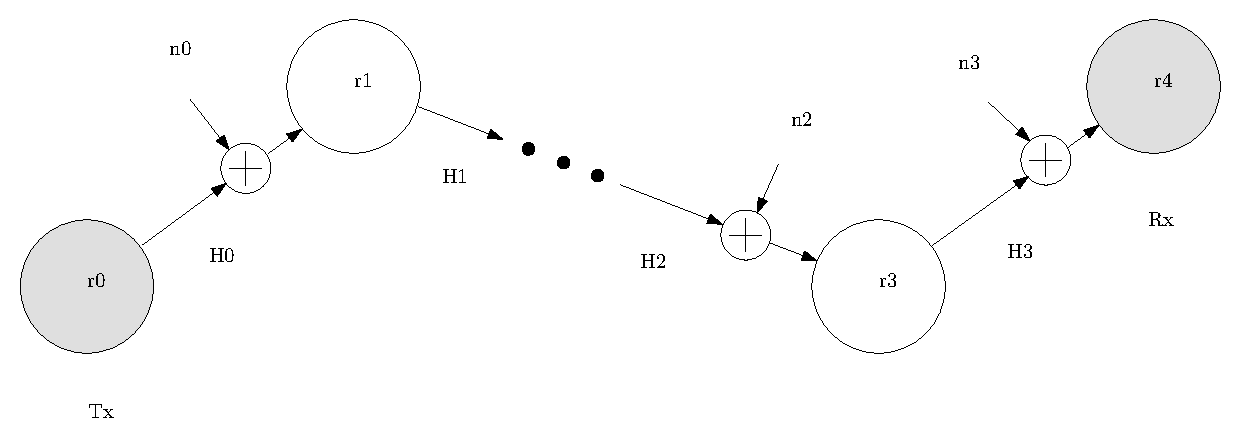
\includegraphics[width=5in]{sp_model.eps}
   \caption{Single Path Relay Network \label{fig:sp_sm} }
\end{figure}

\section{Amplify-and-Forward}
\label{sec:sp_af}

\subsection{System Model}
\label{subsec:sp_af_sm}

Figure \ref{fig:sp_sm} shows the single path relay network.  In the figure, $r_0$ is the transmitter, $r_{m+1}$ is the receiver, and $r_1, \ldots, r_m$ are $m$ relay nodes connected in series forming a single path link between the transmitter and receiver.  The relays perform amplify-and-forward (AF) relaying.  We assume that OFDM with $N$ subcarriers is used in the system.

$h_k^{(0)}, \ldots, h_k^{(m)}$ are the complex subchannel gains at the $k^{\mbox{th}}$ subcarrier in the link, for $k = 1$ to $N$.   $n_k^{(0)}, \ldots, n_k^{(m)}$ are the corresponding noises, which are assumed to be mutually independent, zero-mean, circular symmetric complex Gaussians all with variance $N_0 B / N$, where $N_0$ is the power spectral density of the underlying continuous time noise process and $B$ is the OFDM bandwidth of the system.  Let $p_k^{(0)} = P_{\mbox{tot}} / N$ be the transmitter power on the $k^{\mbox{th}}$ subcarrier, where $P_{\mbox{tot}}$ is the net transmitter power.  Let  $\sqrt{p_k^{(l)}}$ be the amplifying gain used in the amplify-and-forward algorithm at the $l^{\mbox{th}}$ relay, for $l=1$ to $m$.  The $k^{\mbox{th}}$ receive symbol at $r_l$ is amplified by $\sqrt{p_k^{(l)}}$ before it is forwarded to the next node.

Let $x_k$ be the $k^{\mbox{th}}$ transmit symbol with zero mean and unit variance.  Let $y_k$  be the $k^{\mbox{th}}$ receive symbol at the receiver.  Using Figure \ref{fig:sp_sm}, the input-output relation is


\begin{eqnarray}
y_k & = & \left( \prod_{i=0}^m h_k^{(i)} \sqrt{p_k^{(i)}}  \right) x_k + \sum_{j=0}^m 
\left( \prod_{i=j+1}^m h_k^{(i)} \sqrt{p_k^{(i)}}  \right) n_k^{(j)} \mbox{,}
\label{eqn:sp_af_inout}
\end{eqnarray}
where we assume $\prod_{i=q}^{r} a^{(i)} = 1$ for $q > r$ and any $a^{(i)}$.  We use this assumption throughout the rest of this paper.
If we define
\begin{eqnarray}
h_k = \displaystyle\prod_{i=0}^m  h_k^{(i)} \sqrt{p_k^{(i)}}
\mbox{,} & 
\gamma_k^{(j)} = \displaystyle\prod_{i=j+1}^m h_k^{(i)}  \sqrt{p_k^{(i)}}
\mbox{,}
\label{eqn:sp_af_hk_gammak}
\end{eqnarray}
\begin{eqnarray}
\mathbf{\Gamma}_k = \left[
\begin{array}{ccc}
\gamma_k^{(0)} & \cdots & \gamma_k^{(m)}
\end{array}
\right]
\mbox{,} &
\mathbf{n}_k = \left[
\begin{array}{ccc}
n_k^{(0)} & \cdots & n_k^{(m)}
\end{array} \right]^T\mbox{,}
\label{eqn:sp_af_Gammak_nk}
\end{eqnarray}
and
\begin{eqnarray}
w_k = \mathbf{\Gamma}_k \mathbf{n}_k \mbox{,} 
\label{eqn:sp_af_wk}
\end{eqnarray}
then (\ref{eqn:sp_af_inout}) can be written as
\begin{eqnarray}
y_k = h_k x_k + w_k \mbox{.}
\label{eqn:sp_af_inout_terse}
\end{eqnarray}

Now, consider the variance of $w_k$.  Using (\ref{eqn:sp_af_hk_gammak}), (\ref{eqn:sp_af_Gammak_nk}), and (\ref{eqn:sp_af_wk}), we have
\begin{eqnarray}
R_{w_kw_k} & = & E \left[ w_k w_k^* \right] \\
& = & E \left[ \mathbf{\Gamma}_k \mathbf{n}_k \mathbf{n}_k^H \mathbf{\Gamma}_k^H \right] \\
& = & \mathbf{\Gamma}_k E \left[ \mathbf{n}_k \mathbf{n}_k^H  \right] \mathbf{\Gamma}_k^H \\
    & = & \frac{N_0B}{N} \sum_{j=0}^{m} \left( \prod_{i=j+1}^mb_k^{(i)}  p_k^{(i)}  \right) ,
\label{eqn:sp_af_Rwkwk}
\end{eqnarray}
where $E\left[ \cdot \right]$ is the expectation operator, $\left(\cdot\right)^*$ is the complex conjugate operator for a scalar, $\left( \cdot \right)^H$ is the Hermitian (complex transpose) operator for a vector or matrix, and $b_k^{(i)} = \left| h_k^{(i)} \right|^2$, for $i=0$ to $m$.  $R_{w_kw_k}$ is positive for a nonzero $N_0$.  We define a transformed version of the system in (\ref{eqn:sp_af_inout_terse})
\begin{eqnarray}
\tilde{y}_k = \tilde{h}_k x_k + \tilde{w}_k,
\end{eqnarray}
where $\tilde{y}_k = y_k / \sqrt{R_{w_kw_k}}$, $\tilde{h}_k = h_k / \sqrt{R_{w_kw_k}}$, and $\tilde{w}_k = w_k / \sqrt{R_{w_kw_k}}$.  The variances of $\tilde{w}_k$ and $\tilde{y}_k$ are
\begin{eqnarray}
E \left[ \tilde{w}_k \tilde{w}_k^* \right] & = & E \left[ \frac{w_k}{\sqrt{R_{w_kw_k}}} \frac{w_k^*}{\sqrt{R_{w_kw_k}}} \right] \\
& = & \frac{R_{w_kw_k}}{R_{w_kw_k}} \\
& = & 1
\end{eqnarray}
and
\begin{eqnarray}
E \left[ \tilde{y}_k \tilde{y}_k^* \right] & = & E \left[ \left( \tilde{h}_k x_k + \tilde{w}_k \right) \left( \tilde{h}_k x_k + \tilde{w}_k \right)^* \right] \\
& = & \tilde{h}_k \tilde{h}_k^* + 1 \\
& = & \frac{1}{R_{w_kw_k}} \left( \prod_{i=0}^m b_k^{(i)} p_k^{(i)} \right) + 1
\label{eqn:sp_af_yk_tilde_var} \mbox{,}
\end{eqnarray}
respectively.  The cross terms do not appear in (\ref{eqn:sp_af_yk_tilde_var}) because $\tilde{h_k}$, $\tilde{w_k}$, and $x_k$ are mutually independent.  Note that the transformed system has unit variance noise.

\subsection{Mutual Information}
\label{subsec:sp_af_mi}

To derive the mutual information, note that the differential entropy of a circular symmetric complex Gaussian vector, $\mathbf{v}$, with covariance matrix, $\mathbf{K}$, is $h\left(\mathbf{v}\right) = \log_2 \det \left( \pi e \mathbf{K} \right)$ \cite{article:Telatar01}.  When the circular symmetric complex Gaussian is a scalar, $v$, the differential entropy is $h\left(v\right) = \log_2 \left( \pi e \sigma_v^2 \right)$, where $\sigma_v^2$ is the variance of $v$.  Let $\mathcal{I}_k$ be the mutual information between the transmitter and receiver on the $k^{\mbox{th}}$ subcarrier
\begin{eqnarray}
\mathcal{I}_k & = & h\left( \tilde{y}_k \right) - h \left( \tilde{w}_k \right) \\
& = & \log_2 \left( \pi e \left[ \frac{1}{R_{w_kw_k}} \left( \prod_{i=0}^m b_k^{(i)} p_k^{(i)} \right) + 1 \right] \right)
- \log_2 \left( \pi e \right) \\
& = & \log_2 \left[ \frac{1}{R_{w_kw_k}} \left( \prod_{i=0}^m b_k^{(i)} p_k^{(i)} \right) + 1 \right],
\label{eqn:sp_af_Ik}
\end{eqnarray}
where the first equality comes from basic mutual information calculations \cite{book:Cover01}.  The total mutual information between the transmitter and receiver, $\mathcal{I}$, is the sum of all $\mathcal{I}_k$ divided by $N$.  That is, after substituting (\ref{eqn:sp_af_Rwkwk}) into (\ref{eqn:sp_af_Ik}), we have
\begin{eqnarray}
\mathcal{I} & = &\frac{1}{N} \sum_{k=1}^N \mathcal{I}_k\\
& = &\frac{1}{N} \sum_{k=1}^N \log_2 \left( 1 + \mbox{SNR}
\left[ \frac{b_k^{(0)}\left( \prod_{i=1}^m b_k^{(i)}  p_k^{(i)}  \right)}
{\sum_{j=0}^m \left( \prod_{i=j+1}^m b_k^{(i)}  p_k^{(i)}  \right) }\right]
 \right),
\label{eqn:sp_af_I}
\end{eqnarray}
where $\mbox{SNR} = P_{\mbox{tot}} / N_0 B$.  If we denote
\begin{eqnarray}
\begin{array}{ccc}
\mathbf{b}^{(i)} = \left[ \begin{array}{ccc}
b_1^{(i)} & \cdots & b_N^{(i)}
\end{array}
\right]^T &  \mbox{and} &   
\mathbf{p}^{(i)} = \left[ \begin{array}{ccc}
p_1^{(i)} & \cdots & p_N^{(i)}
\end{array}
\right]^T,
\end{array} 
\end{eqnarray} 
for $i = 0$ to $m$ and
\begin{eqnarray}
\mathbf{e}_N = \underbrace{ \left[ \begin{array}{ccc}
1 & \cdots & 1
\end{array}
\right]^T}_{\mbox{$N$ ones}},
\end{eqnarray}
then (\ref{eqn:sp_af_I}) can be written in matrix form.  First, let
\begin{eqnarray}
\mathbf{z}_{\mbox{single}} = \left[ \mathbf{b}^{(0)} \circ \left( \circ \prod_{i=1}^m \mathbf{b}^{(i)} \circ  \mathbf{p}^{(i)}  \right) \right] \circ / 
\left[ \sum_{j=0}^{m} \left(\circ \prod_{i=j+1}^{m}  \mathbf{b}^{(i)} \circ \mathbf{p}^{(i)} \right) \right],
\end{eqnarray}
where the $\circ$ and $\circ \prod$ operators both represent element-wise matrix multiplication and the $\circ /$ operator represents element-wise matrix division.  Then, (\ref{eqn:sp_af_I}) in matrix form is
\begin{eqnarray}
\mathcal{I} = \frac{1}{N}\mathbf{e}_N^T  \log_2 \left( \mathbf{e}_N + \mbox{SNR} \: \mathbf{z}_{\mbox{single}} \right),
\label{eqn:sp_af_I_matrix}
\end{eqnarray}
where $\log_2\left( \cdot \right)$ of a vector is the vector of the logarithms of the vector's entries.

\subsection{Relay Power Allocation}
\label{subsec:sp_af_rpa}

We assume that the net transmit power at the transmitter and at each each relay is $P_{\mbox{tot}}$.  At the transmitter, we assume a uniform power distribution, that is, $p_k^{(0)} = P_{\mbox{tot}}/N$.  To derive the power constraint at each relay and thus, possible power allocations, consider $v_k^{(l)}$, the $k^{\mbox{th}}$ transmit symbol of $r_l$
\begin{eqnarray}
v_k^{(l)} = \sqrt{p_k^{(l)}} \left[ \left( \prod_{i=0}^{l-1} h_k^{(i)}  \sqrt{p_k^{(i)}} \right)  x_k + \sum_{j=0}^{l-1}\left( \prod_{i=j+1}^{l-1} h_k^{(i)}  \sqrt{p_k^{(i)}} \right)n_k^{(j)} \right] \mbox{.}
\end{eqnarray}
The constraint is $P_{\mbox{tot}} = \displaystyle \sum_{k=1}^{N} E \left[ \left| v_k^{(l)} \right|^2 \right]$.  Thus,
\begin{eqnarray}
P_{\mbox{tot}} = \displaystyle \sum_{k=1}^{N} p_k^{(l)}
\left[ b_k^{(0)} \frac{P_{\mbox{tot}}}{N}  \left( \displaystyle \prod_{i=1}^{l-1}  b_k^{(i)} p_k^{(i)} \right) + 
\frac{N_0 B}{N} \sum_{j=0}^{l-1} \left( \displaystyle \prod_{i=j+1}^{l-1}  b_k^{(i)} p_k^{(i)} \right) 
\right]
\label{eqn:sp_af_powerconstraint0}
\end{eqnarray}
or
\begin{eqnarray}
\sum_{k=1}^N \frac{ p_k^{(l)}}{N} \left[
b_k^{(0)} \left( \prod_{i=1}^{l-1}  b_k^{(i)}p_k^{(i)} \right) + 
\frac{1}{\mbox{SNR}} \sum_{j=0}^{l-1} \left( \prod_{i=j+1}^{l-1}  b_k^{(i)}p_k^{(i)}
\right)
\right] =1.
\label{eqn:sp_af_powerconstraint}
\end{eqnarray}
Note that (\ref{eqn:sp_af_powerconstraint}) is defined recursively.  The power constraint for $p_k^{(l)}$ depends on $p_k^{(1)}, \dots, p_k^{(l-1)}$.  $p_k^{(1)}$ is the base case in the recursion, which follows from (\ref{eqn:sp_af_powerconstraint}), when $l = 1$.

One power allocation at the $l^{\mbox{th}}$ relay is to set $p_k^{(l)}$ constant for all subcarriers.  This results in moving $p_k^{(l)}$ in (\ref{eqn:sp_af_powerconstraint}) out of the summation because it is no longer a function of $k$
\begin{eqnarray}
p_{k,ct}^{(l)} = p_{ct}^{(l)} = 
 \frac{N \mbox{SNR}}
{\displaystyle \sum_{k=1}^N \left[ \mbox{SNR} b_k^{(0)} \left( \displaystyle \prod_{i=1}^{l-1} b_k^{(i)} p_{ct}^{(i)}\right) + \displaystyle \sum_{j=0}^{l-1} \left( \displaystyle \prod_{i=j+1}^{l-1} b_k^{(i)} p_{ct}^{(i)}\right)
\right]
} \mbox{.}
\end{eqnarray}
We call this \emph{constant gain allocation} (CT).  Note that this power allocation does not require each relay to have any CSI (channel state information).  The $l^{\mbox{th}}$ relay only has to multiply its entire OFDM receive symbol by a constant, $\sqrt{p_{ct}^{(l)}}$, such that the total transmit power is $P_{\mbox{tot}}$.  We call \emph{constant gain capacity}, $C_{ct}$, as the mutual information in (\ref{eqn:sp_af_I_matrix}) resulting from this power allocation.

A second power allocation is to choose $p_k^{(l)}$ such that every subcarrier transmits the same power at the $l^{\mbox{th}}$ relay.  The transmit power on the $k^{\mbox{th}}$ subcarrier is the $k^{\mbox{th}}$ summand on the right hand side of (\ref{eqn:sp_af_powerconstraint0}).  Since they are all equal to $P_{\mbox{tot}}/N$, we have
\begin{eqnarray}
\frac{P_{\mbox{tot}}}{N} = 
 p_{k,eq}^{(l)}
\left[b_k^{(0)} \frac{P_{\mbox{tot}}}{N}  \left( \displaystyle \prod_{i=1}^{l-1} b_k^{(i)} p_{k,eq}^{(i)} \right) + 
\frac{N_0 B}{N} \sum_{j=0}^{l-1} \left( \displaystyle \prod_{i=j+1}^{l-1} b_k^{(i)} p_{k,eq}^{(i)} \right) 
\right]\end{eqnarray}
or
\begin{eqnarray}
p_{k,eq}^{(l)} = \frac{\mbox{SNR}}
{\mbox{SNR} b_k^{(0)} \left( \displaystyle\prod_{i=1}^{l-1}b_k^{(i)} p_{k,eq}^{(i)} \right) + \displaystyle\sum_{j=0}^{l-1} \left(
\prod_{i=j+1}^{l-1}  b_k^{(i)} p_{k,eq}^{(i)}
\right)} \mbox{.}
\label{}
\end{eqnarray}
We call this \emph{equal power allocation} (EQ).  Note that this power allocation does require each relay to have the CSI of its upstream channels.  We call \emph{equal power capacity}, $C_{eq}$, as the mutual information in (\ref{eqn:sp_af_I_matrix}) resulting from this power allocation.

\subsection{Capacity Simulations}
\label{subsec:sp_af_cs}

We simulate $C_{ct}$ and $C_{eq}$ assuming that all distances between any two adjacent transceiver nodes are the same.  Therefore, all path loss effects are normalized to $0$ dB.  Shadowing between nodes is assumed to be log-normally distributed.  That is, the received power gain due to shadowing in dB is a zero-mean Gaussian with variance of 8 dB, which is typical for cellular land mobile applications \cite{book:Stuber01}.  We model frequency selective fading effects as Typical Urban (TU) channels and Hilly Terrain (HT) channels \cite{book:Stuber01}.  We use an OFDM bandwidth of 800 kHz divided into $N=128$ equal blocks.  Maintaining OFDM orthogonality, this translates into an OFDM symbol period of $T_s = 160\:\mu$s.  Results are shown in Figures \ref{fig:sp_af_cap_plots_TU} and  \ref{fig:sp_af_cap_plots_HT}.

The plots exhibit the familiar monotonically increasing shape for mutual information in the case of direct transmission between a transmitter and receiver.  This is expected if we look at the mutual information in (\ref{eqn:sp_af_I_matrix}).  We can think of this configuration as still being direct transmission where the channel is the single path relay network, characterized by $\mathbf{z}_{\mbox{single}}$.  Note that $\mathbf{z}_{\mbox{single}}$ also determines the power allocations in the relays.  In other words, (\ref{eqn:sp_af_I_matrix}) is a system level representation of the mutual information.

As we increase the distance between the transmitter and receiver (and thus, add more relays), more noise and channel distortion enter the system.  Consequently, the mutual information decreases.  Equal power allocation results in a slightly higher mutual information than that of constant gain allocation.  TU channels and HT channels give very similar results.

\begin{figure*}
    \psfrag{Capacity}[Bc][tc][0.8]{Capacity (bits/s/Hz)}
    \psfrag{SNR}[tc][Bc][0.8]{SNR (dB)}
    \psfrag{Cct-}[cl][cl][0.6]{$C_{ct}$}
    \psfrag{Ceq-}[cl][cl][0.6]{$C_{eq}$}
    \psfrag{Caa-}[cl][cl][0.6]{$C_{aa}$}
\centerline{
	\subfigure[m=1]{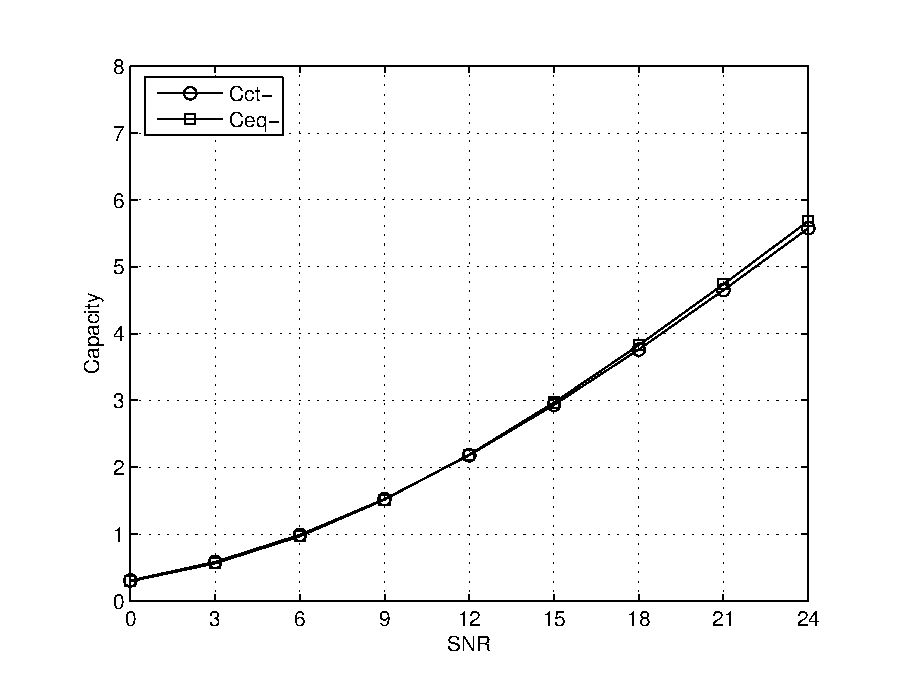
\includegraphics[width=3in]{sp_af_cap_m1_TU.eps} \label{}} 
	\subfigure[m=2]{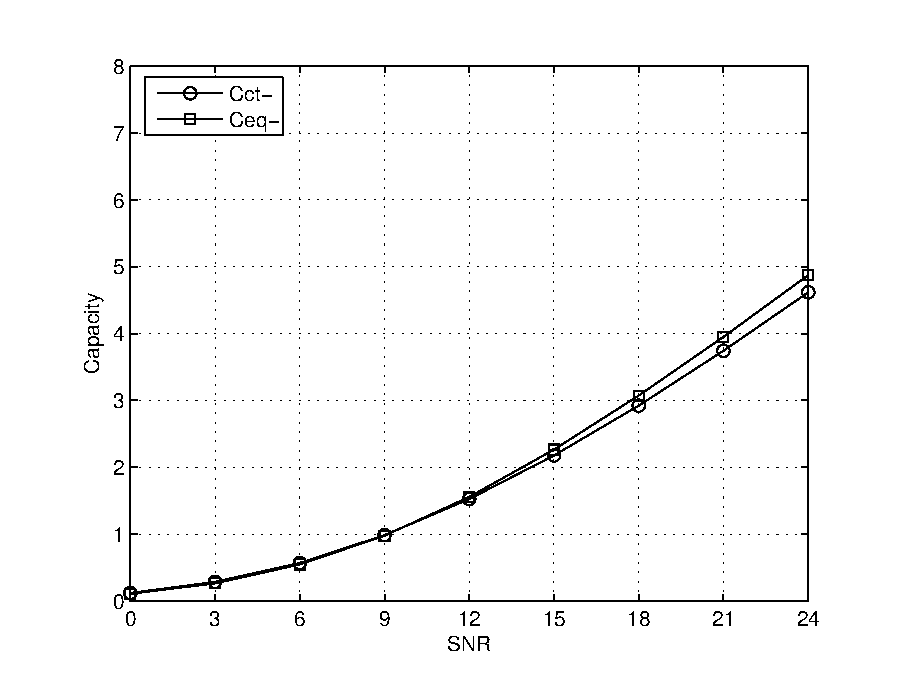
\includegraphics[width=3in]{sp_af_cap_m2_TU.eps} \label{}} \\
}
\centerline{
	\subfigure[m=3]{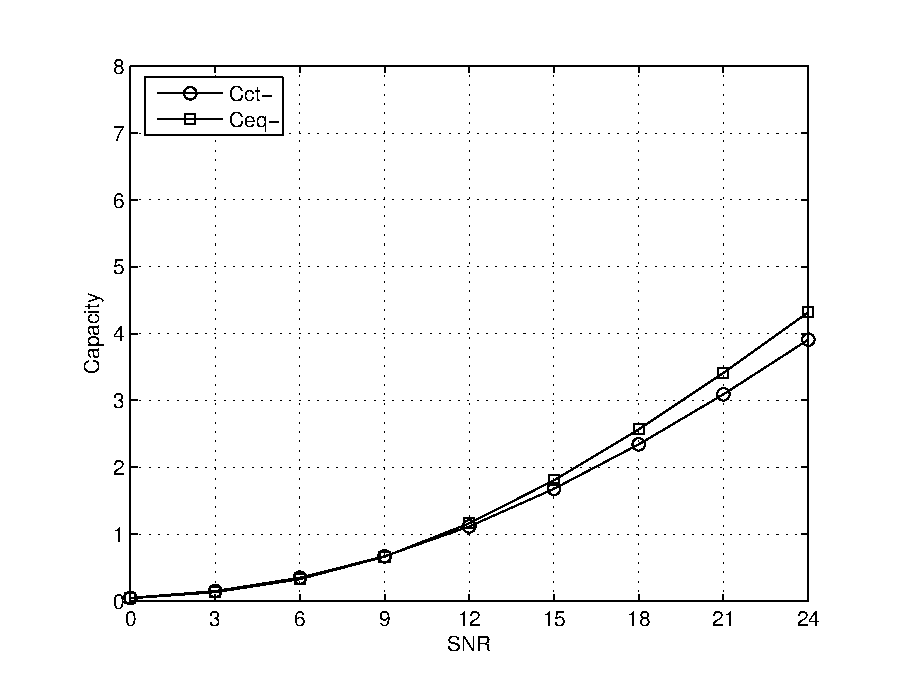
\includegraphics[width=3in]{sp_af_cap_m3_TU.eps} \label{}}
	\subfigure[m=4]{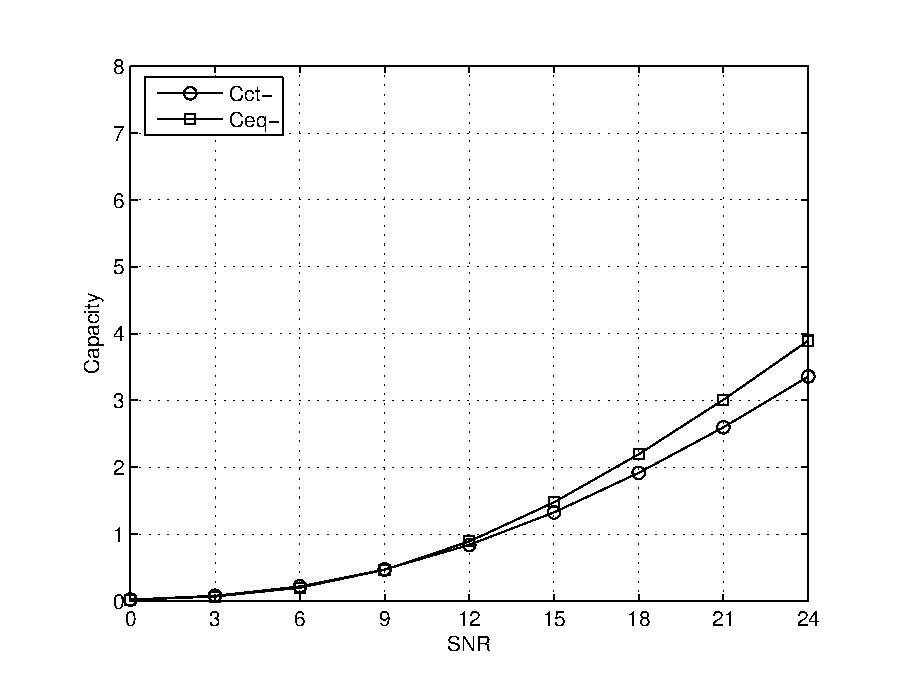
\includegraphics[width=3in]{sp_af_cap_m4_TU.eps} \label{}} \\
}
\caption{Capacity in a single path relay network with TU channels using AF.  $N = 128, m = 1, 2, 3$, and $4$.}
\label{fig:sp_af_cap_plots_TU}
\end{figure*}

\begin{figure*}
    \psfrag{Capacity}[Bc][tc][0.8]{Capacity (bits/s/Hz)}
    \psfrag{SNR}[tc][Bc][0.8]{SNR (dB)}
    \psfrag{Cct-}[cl][cl][0.6]{$C_{ct}$}
    \psfrag{Ceq-}[cl][cl][0.6]{$C_{eq}$}
    \psfrag{Caa-}[cl][cl][0.6]{$C_{aa}$}
\centerline{
	\subfigure[m=1]{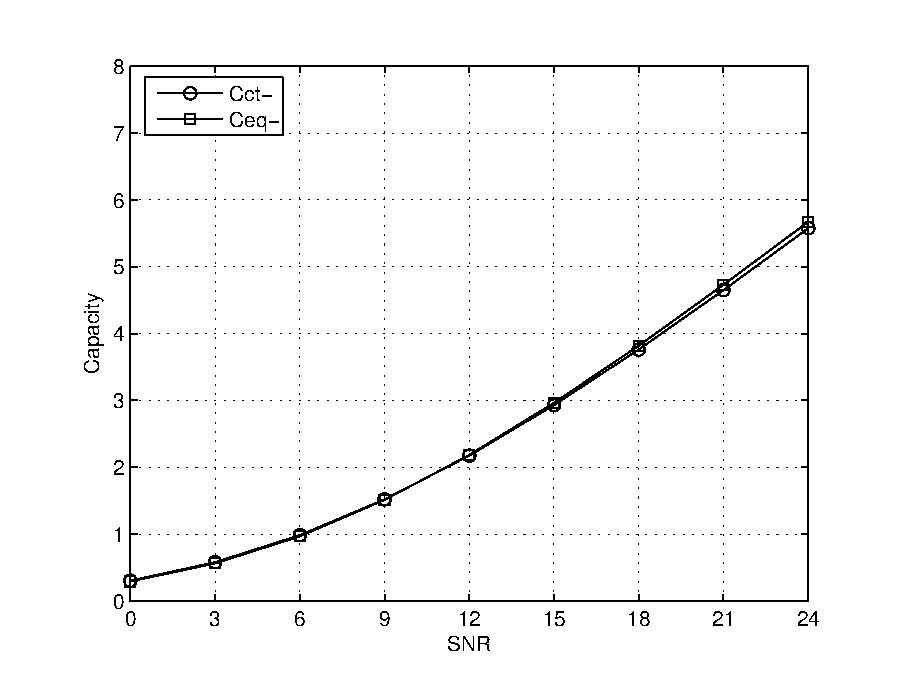
\includegraphics[width=3in]{sp_af_cap_m1_HT.eps} \label{}} 
	\subfigure[m=2]{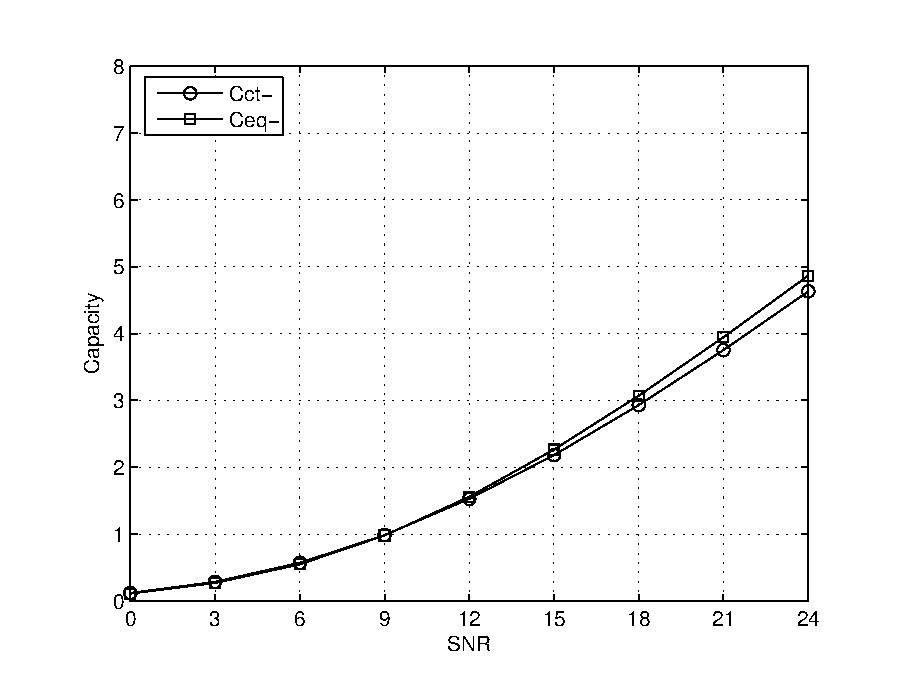
\includegraphics[width=3in]{sp_af_cap_m2_HT.eps} \label{}} \\
}
\centerline{
	\subfigure[m=3]{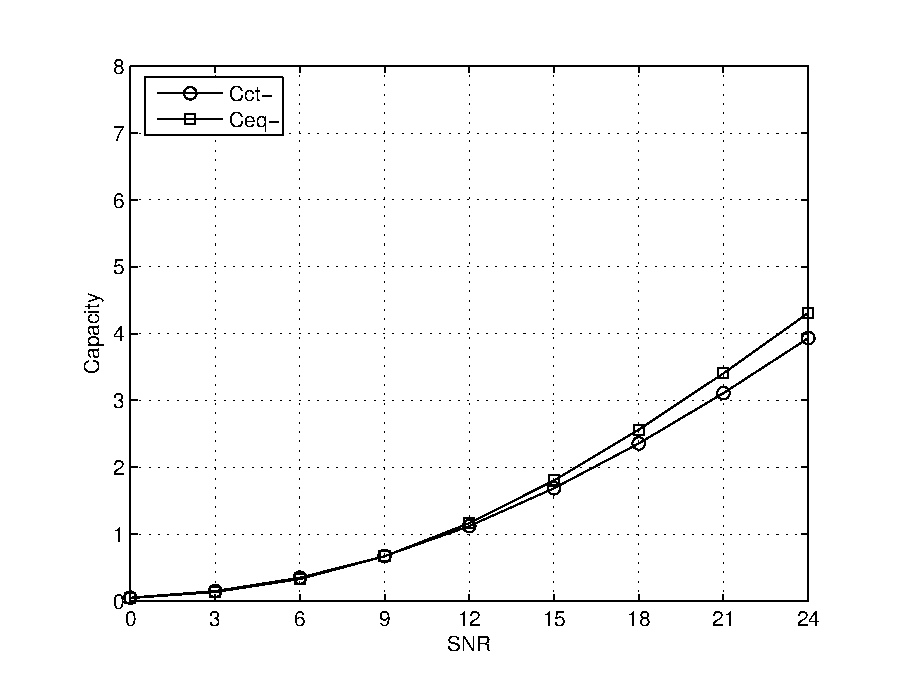
\includegraphics[width=3in]{sp_af_cap_m3_HT.eps} \label{}}
	\subfigure[m=4]{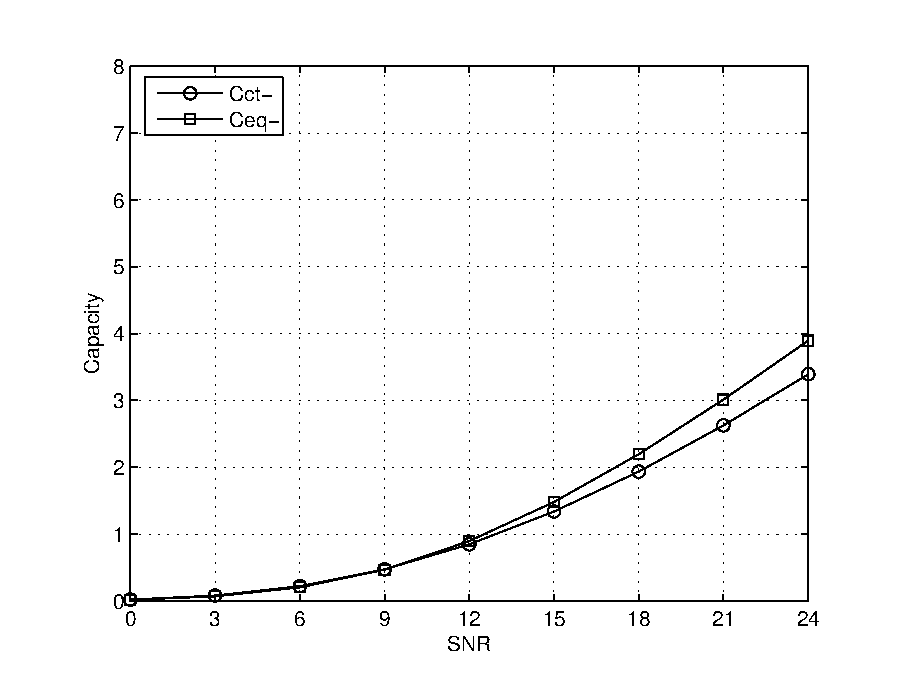
\includegraphics[width=3in]{sp_af_cap_m4_HT.eps} \label{}} \\
}
\caption{Capacity in a single path relay network with HT channels using AF.  $N = 128, m = 1, 2, 3$, and $4$.}
\label{fig:sp_af_cap_plots_HT}
\end{figure*}


\section{Decode-and-Forward}
\label{sec:sp_df}

\subsection{System Model}
\label{subsec:sp_df_sm}

In decode-and-forward (DF), each relay fully recovers the information bits (with possible errors) after receiving an OFDM symbol.  It then converts the information bits back into an OFDM symbol and then transmits it.  The transmitter and all the relays transmit with the same uniform power distribution.  That is,
\begin{eqnarray}
p_k^{(0)} = p_k^{(l)} = \frac{P_{\mbox{tot}}}{N}\mbox{,}
\end{eqnarray}
for $k = 1$ to $N$ and for $l = 1$ to $m$.

Let $x_k^{(0)}$ be the $k^{\mbox{th}}$ transmit symbol from the transmitter and  $x_k^{(l)}$ be the $k^{\mbox{th}}$ transmit symbol from the $l^{\mbox{th}}$ relay, all with with zero mean and unit variance.  Let $y_k^{(m+1)}$ be the $k^{\mbox{th}}$ receive symbol at the receiver and  $y_k^{(l)}$ be the $k^{\mbox{th}}$ receive symbol at the $l^{\mbox{th}}$ relay.  Using Figure \ref{fig:sp_sm}, the input-ouput relation at the $l^{\mbox{th}}$ relay is
\begin{eqnarray}
y_k^{(l)} = h_k^{(l-1)} \sqrt{\frac{P_{\mbox{tot}}}{N}} x_k^{(l-1)} + n_k^{(l-1)} \mbox{.}
\end{eqnarray}
The input-output relation at the receiver is
\begin{eqnarray}
y_k^{(m+1)} =h_k^{(m)}  \sqrt{\frac{P_{\mbox{tot}}}{N}} x_k^{(m)} + n_k^{(m)} \mbox{.}
\end{eqnarray}

\section{BER and WER Simulations}
\label{sec:sp_bws}

\begin{figure}
  \centering
    \psfrag{in}[cr][cc][0.9]{input}
    \psfrag{o1}[cl][Bl][0.9]{output 1}
    \psfrag{o2}[cl][Bl][0.9]{output 2}
    \psfrag{o3}[cl][Bl][0.9]{output 3}
    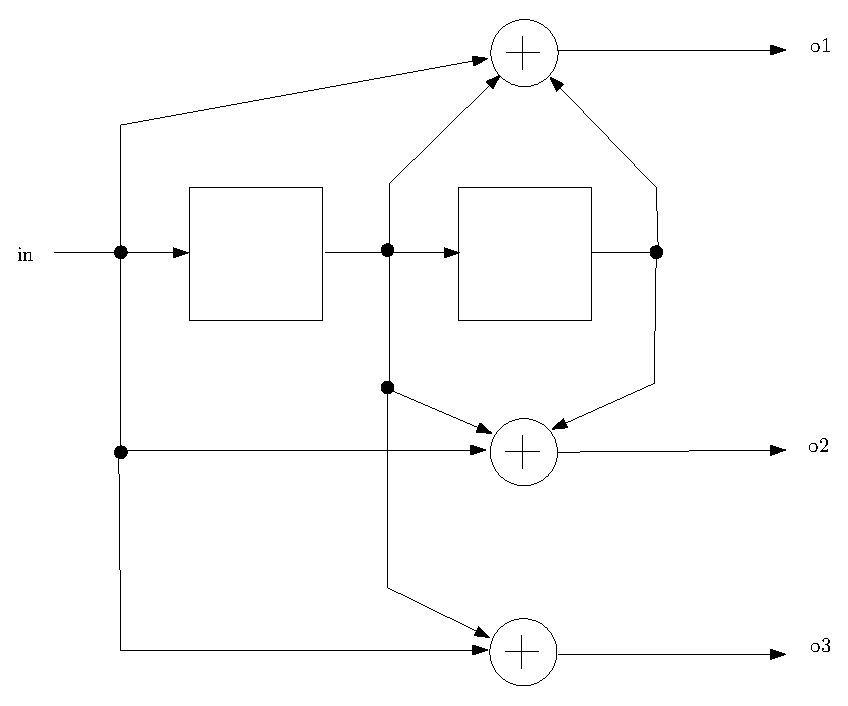
\includegraphics[width=4in]{conv_enc.eps}
   \caption{Convolutional encoder. \label{fig:conv_enc} }
\end{figure}

We simulate bit error rates (BERs) and word error rates (WERs) for both the amplify-and-forward and decode-and-forward cases.  At the transmitter (and at the transmitter structure of a relay using decode-and-forward), each information word contains 83 bits.  Using the convolutional encoder shown in Figure \ref{fig:conv_enc}, the information word is encoded into a 255 bit codeword.  A zero bit is padded at the end to make 256 bits.  The bits are then interleaved and modulated onto $N = 128$ QPSK (quadrature phase shift keying) subcarriers to form one OFDM symbol.  At the receiver (and at the receiver structure of a relay using decode-and-forward), the codeword is recovered (with possible errors) using a matched filter and deinterleaving.  A Viterbi decoder is used to decode the codeword.  Both hard decisions and soft decisions are used.

We assume that all distances between any two adjacent transceiver nodes are the same.  Therefore, all path loss effects are normalized to 0 dB.  Shadowing is assumed to be log-normally distributed.  That is, the received power gain due to shadowing in dB is a zero-mean Gaussian with variance of 8 dB, which is typical for cellular land mobile applications \cite{book:Stuber01}.  We model frequency selective fading as Typical Urban (TU) channels and Hilly Terrain (HT) channels \cite{book:Stuber01}.  We use an OFDM bandwidth of 800 kHz divided into $N = 128$ equal blocks.  Maintaining OFDM orthogonality, this translates into an OFDM symbol period of $T_s = 160 \:\mu$s.  

\subsection{Amplify-and-Forward}
\label{subsec:sp_bws_af}

The BER versus SNR and WER versus SNR plots for a single path relay network with TU channels using amplify-and-forward are shown in Figures \ref{fig:sp_af_ber_plots_TU} and \ref{fig:sp_af_wer_plots_TU}, respectively.  The corresponding plots for HT channels are shown in Figures \ref{fig:sp_af_ber_plots_HT} and \ref{fig:sp_af_wer_plots_HT}, respectively.

As expected, soft decisions in Viterbi decoding give better performance than hard decisions.  In particular, there is up to 4 dB of SNR gain for the constant gain allocation and $m=1$ case, as shown in Figures \ref{fig:sp_af_ber_m1_TU}, \ref{fig:sp_af_wer_m1_TU}, \ref{fig:sp_af_ber_m1_HT}, and \ref{fig:sp_af_wer_m1_HT}.  In general, using hard decisions with constant gain allocation results in the worst performance.  Soft decisions with equal power allocation gives the best performance, except for the $m=1$ case, where soft decisions with constant gain allocation is slightly better.  

As we increase the distance between the transmitter and receiver (and thus, add more relays), more noise and channel distortion enter the system.  Consequently, the error rate (BER and WER) performance becomes worse and as a result, all four curves are very close together at low to medium SNR values.  TU channels and HT channels give very similar results.

\begin{figure*}
    \psfrag{BER}[Bc][tc][0.8]{BER}
    \psfrag{SNR}[tc][Bc][0.8]{SNR (dB)}
    \psfrag{hard--constant-gain-allocation}[cl][cl][0.5]{hard, constant gain allocation}
    \psfrag{hard--equal-power-allocation}[cl][cl][0.5]{hard, equal power allocation}
    \psfrag{soft--constant-gain-allocation}[cl][cl][0.5]{soft, constant gain allocation}
    \psfrag{soft--equal-power-allocation}[cl][cl][0.5]{soft, equal power allocation}

\centerline{
	\subfigure[m=1]{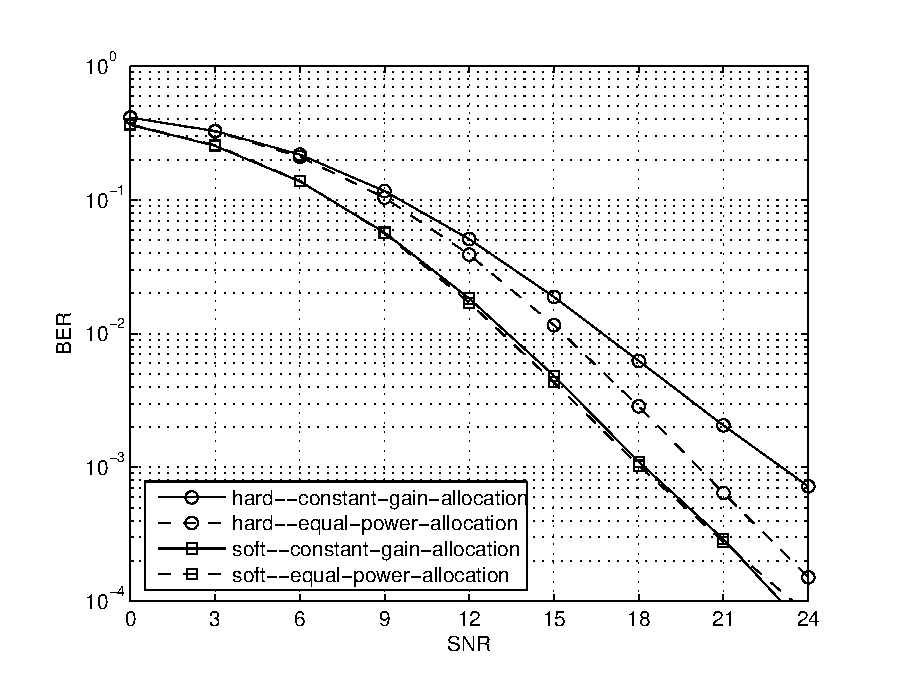
\includegraphics[width=3in]{sp_af_ber_m1_TU.eps} \label{fig:sp_af_ber_m1_TU}} 
	\subfigure[m=2]{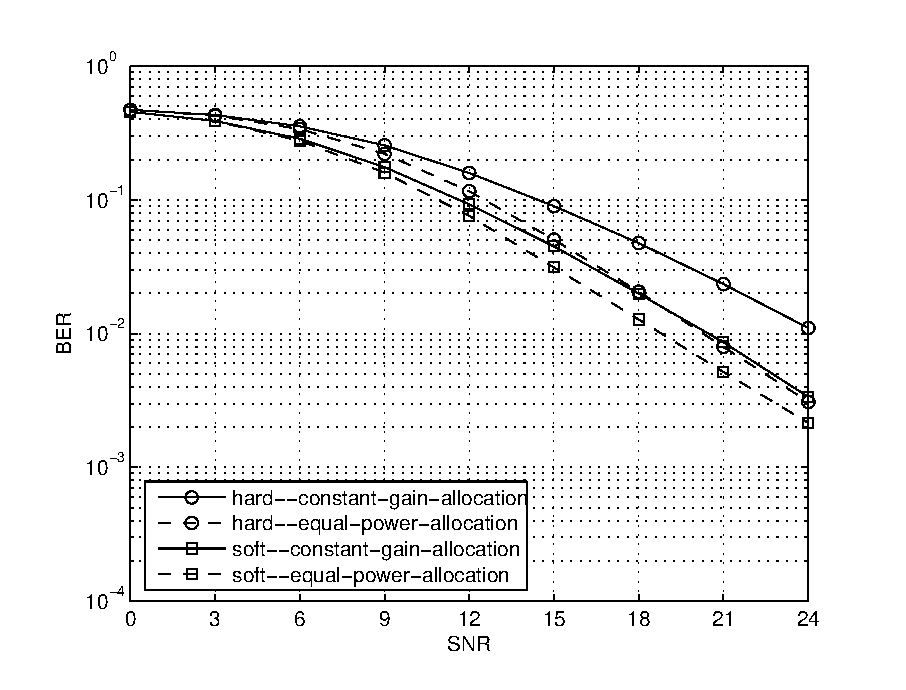
\includegraphics[width=3in]{sp_af_ber_m2_TU.eps} \label{}} \\
}
\centerline{
	\subfigure[m=3]{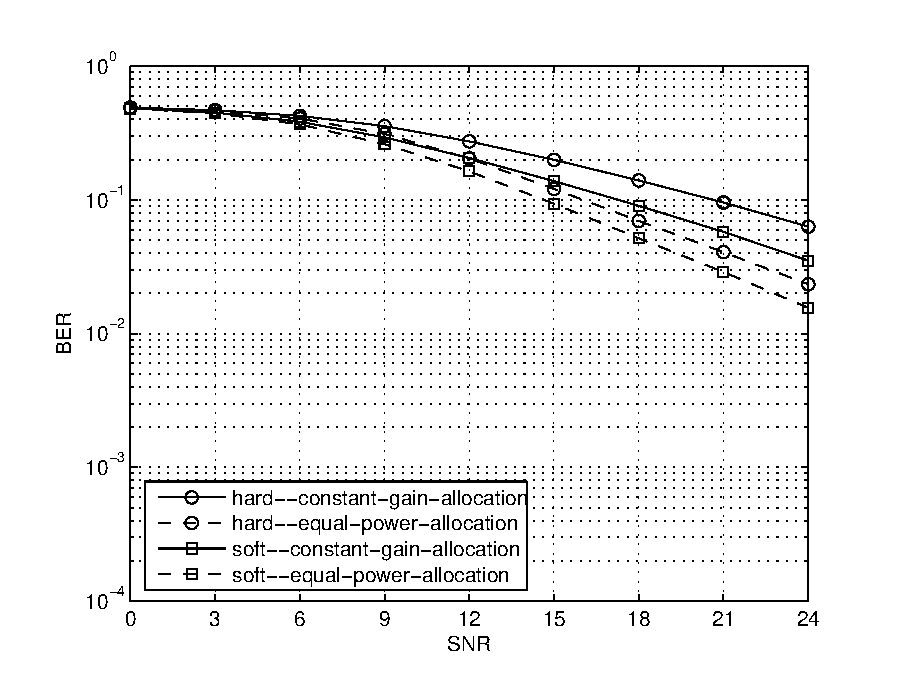
\includegraphics[width=3in]{sp_af_ber_m3_TU.eps} \label{}}
	\subfigure[m=4]{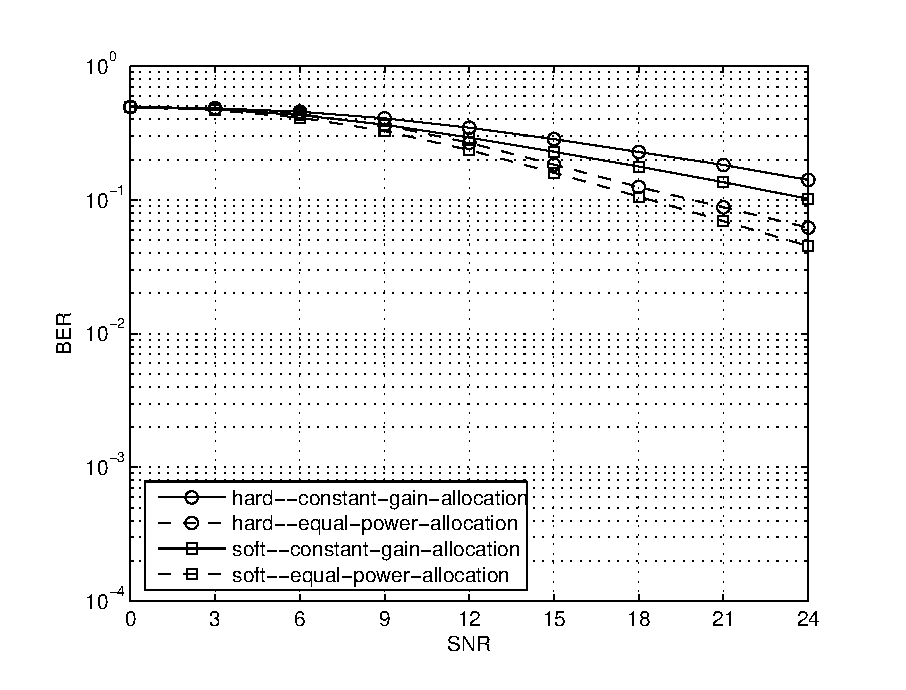
\includegraphics[width=3in]{sp_af_ber_m4_TU.eps} \label{}} \\
}
\caption{BER in a single path relay network with TU channels using AF.  $N = 128, m = 1, 2, 3$, and $4$.}
\label{fig:sp_af_ber_plots_TU}
\end{figure*}

\begin{figure*}
    \psfrag{WER}[Bc][tc][0.8]{WER}
    \psfrag{SNR}[tc][Bc][0.8]{SNR (dB)}
    \psfrag{hard--constant-gain-allocation}[cl][cl][0.5]{hard, constant gain allocation}
    \psfrag{hard--equal-power-allocation}[cl][cl][0.5]{hard, equal power allocation}
    \psfrag{soft--constant-gain-allocation}[cl][cl][0.5]{soft, constant gain allocation}
    \psfrag{soft--equal-power-allocation}[cl][cl][0.5]{soft, equal power allocation}

\centerline{
	\subfigure[m=1]{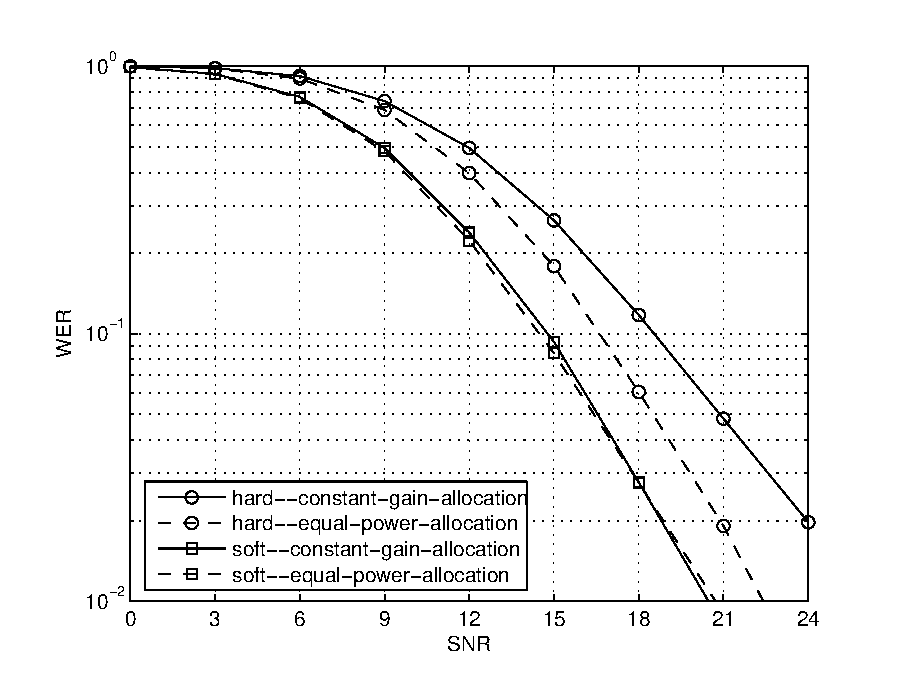
\includegraphics[width=3in]{sp_af_wer_m1_TU.eps} \label{fig:sp_af_wer_m1_TU}} 
	\subfigure[m=2]{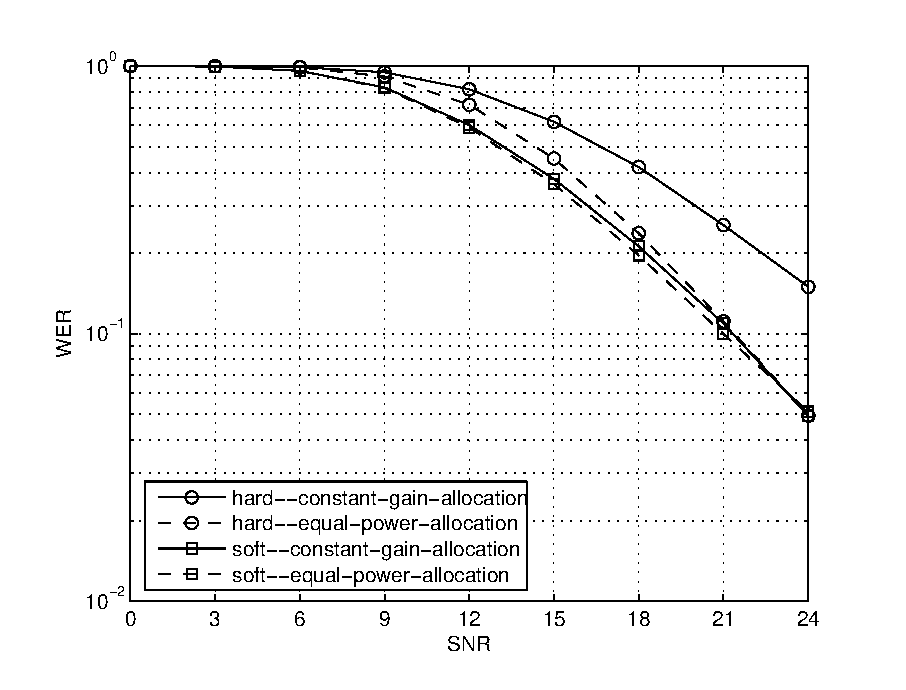
\includegraphics[width=3in]{sp_af_wer_m2_TU.eps} \label{}} \\
}
\centerline{
	\subfigure[m=3]{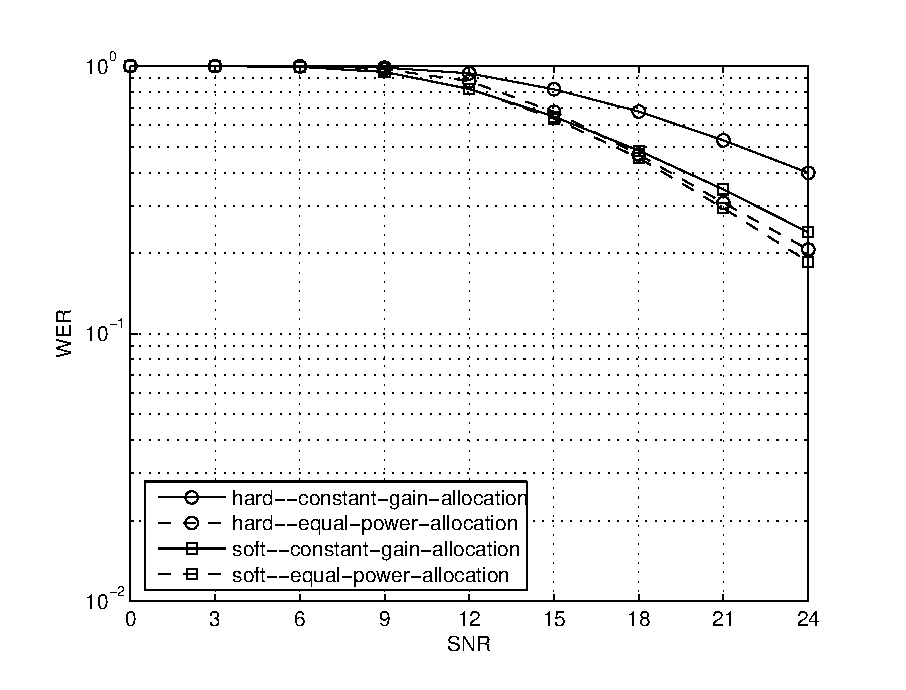
\includegraphics[width=3in]{sp_af_wer_m3_TU.eps} \label{}}
	\subfigure[m=4]{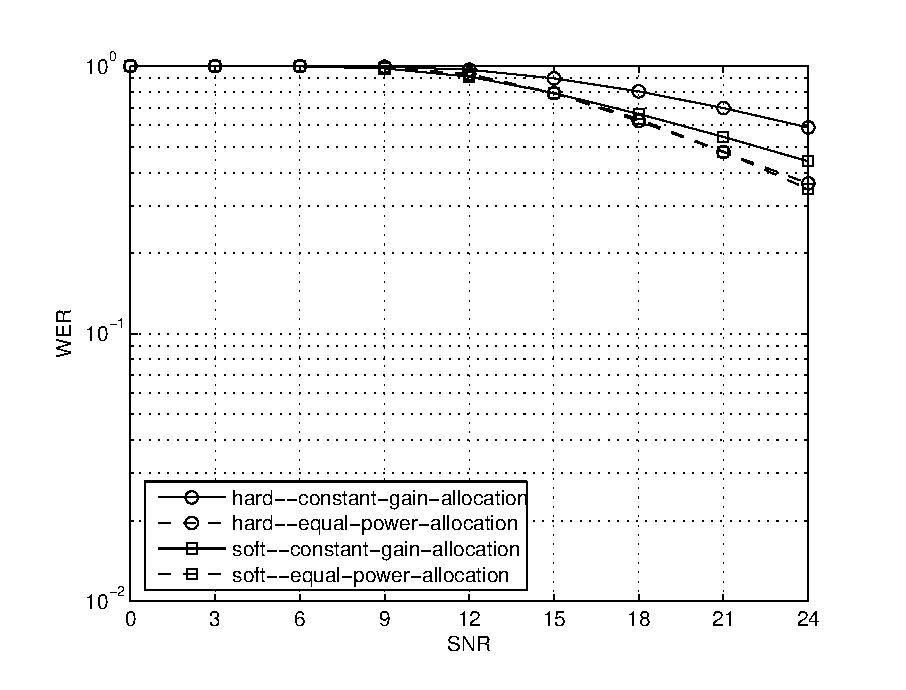
\includegraphics[width=3in]{sp_af_wer_m4_TU.eps} \label{}} \\
}
\caption{WER in a single path relay network with TU channels using AF.  $N = 128, m = 1, 2, 3$, and $4$.}
\label{fig:sp_af_wer_plots_TU}
\end{figure*}

\begin{figure*}
    \psfrag{BER}[Bc][tc][0.8]{BER}
    \psfrag{SNR}[tc][Bc][0.8]{SNR (dB)}
    \psfrag{hard--constant-gain-allocation}[cl][cl][0.5]{hard, constant gain allocation}
    \psfrag{hard--equal-power-allocation}[cl][cl][0.5]{hard, equal power allocation}
    \psfrag{soft--constant-gain-allocation}[cl][cl][0.5]{soft, constant gain allocation}
    \psfrag{soft--equal-power-allocation}[cl][cl][0.5]{soft, equal power allocation}

\centerline{
	\subfigure[m=1]{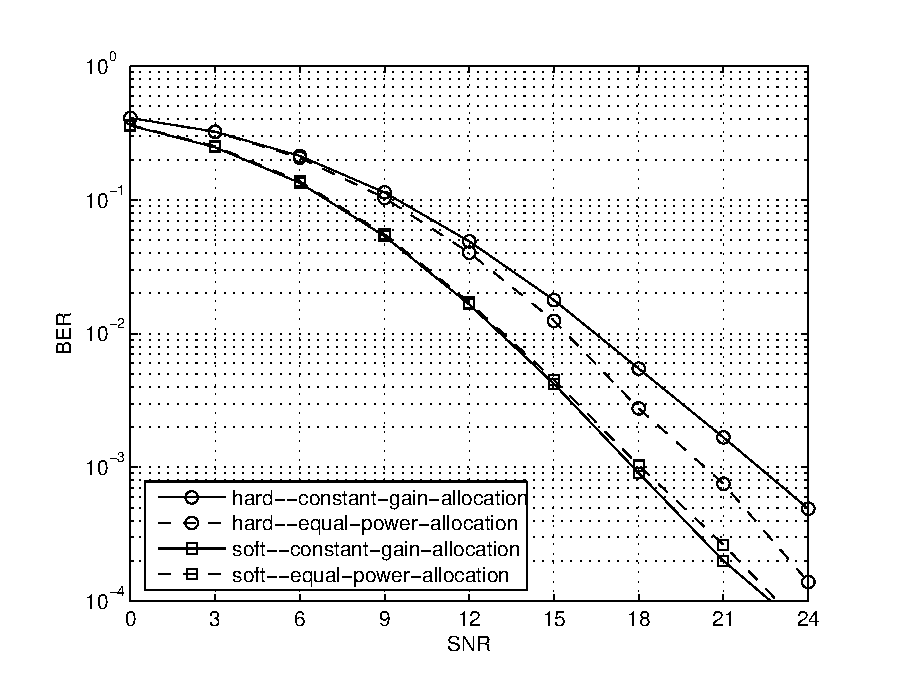
\includegraphics[width=3in]{sp_af_ber_m1_HT.eps} \label{fig:sp_af_ber_m1_HT}} 
	\subfigure[m=2]{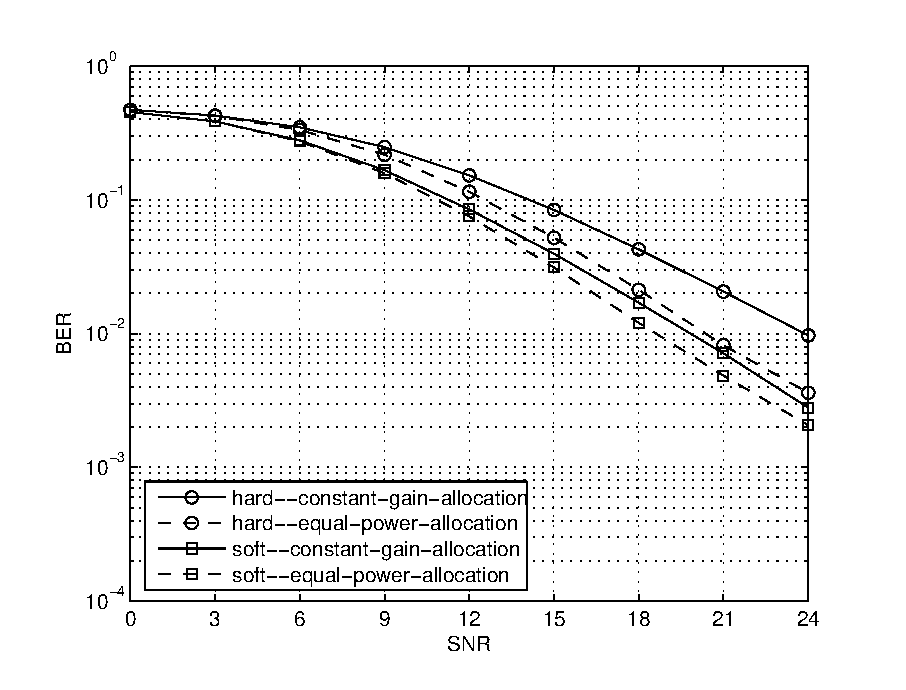
\includegraphics[width=3in]{sp_af_ber_m2_HT.eps} \label{}} \\
}
\centerline{
	\subfigure[m=3]{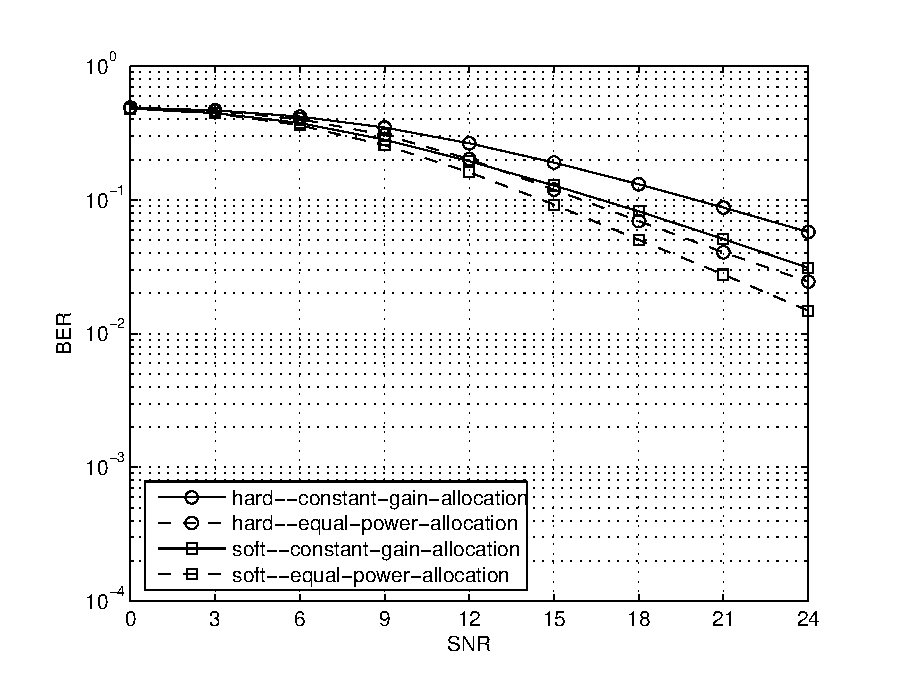
\includegraphics[width=3in]{sp_af_ber_m3_HT.eps} \label{}}
	\subfigure[m=4]{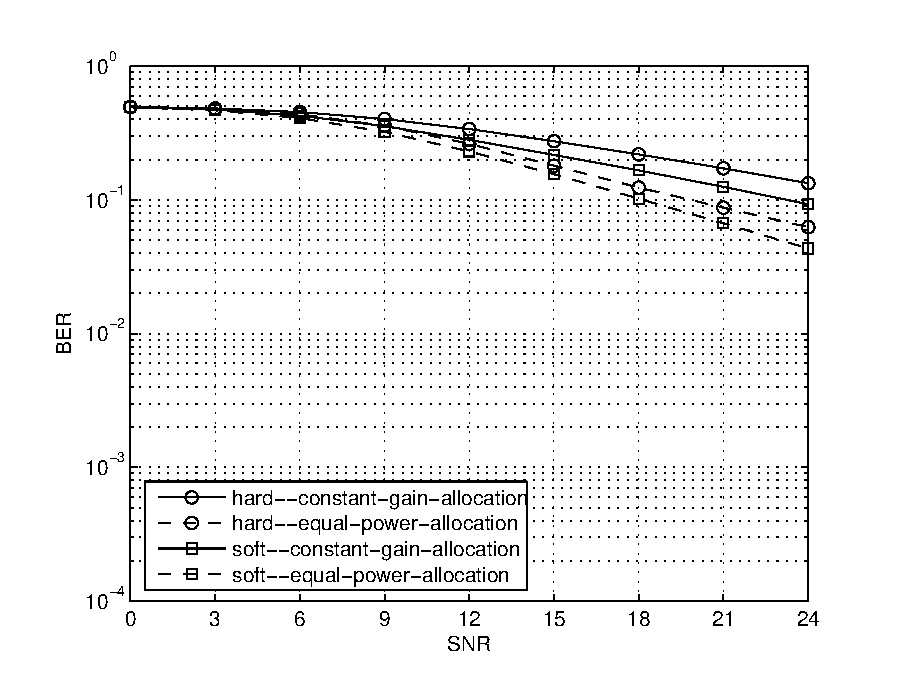
\includegraphics[width=3in]{sp_af_ber_m4_HT.eps} \label{}} \\
}
\caption{BER in a single path relay network with HT channels using AF.  $N = 128, m = 1, 2, 3$, and $4$.}
\label{fig:sp_af_ber_plots_HT}
\end{figure*}

\begin{figure*}
    \psfrag{WER}[Bc][tc][0.8]{WER}
    \psfrag{SNR}[tc][Bc][0.8]{SNR (dB)}
    \psfrag{hard--constant-gain-allocation}[cl][cl][0.5]{hard, constant gain allocation}
    \psfrag{hard--equal-power-allocation}[cl][cl][0.5]{hard, equal power allocation}
    \psfrag{soft--constant-gain-allocation}[cl][cl][0.5]{soft, constant gain allocation}
    \psfrag{soft--equal-power-allocation}[cl][cl][0.5]{soft, equal power allocation}

\centerline{
	\subfigure[m=1]{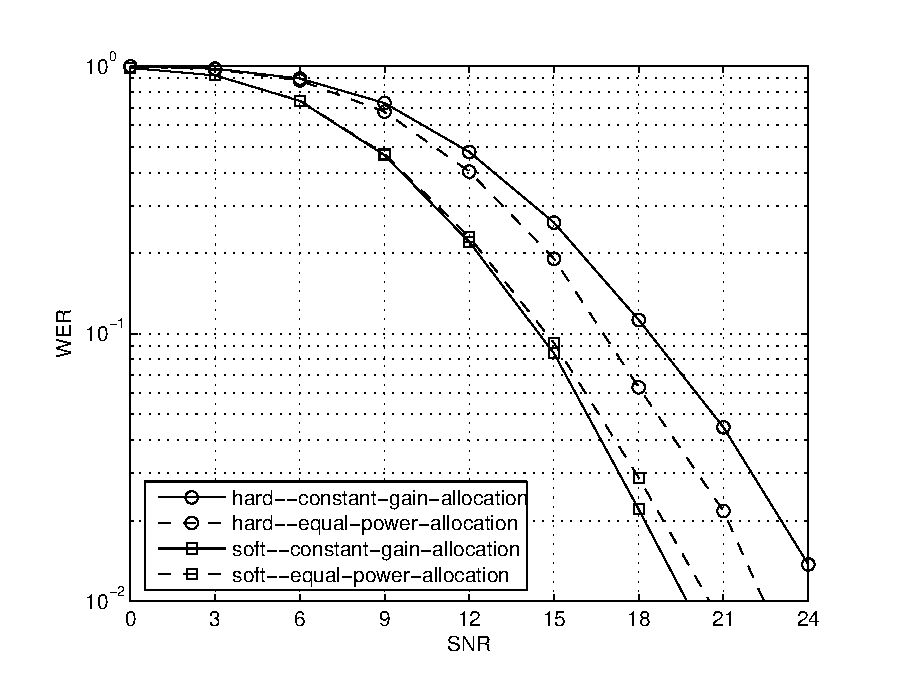
\includegraphics[width=3in]{sp_af_wer_m1_HT.eps} \label{fig:sp_af_wer_m1_HT}} 
	\subfigure[m=2]{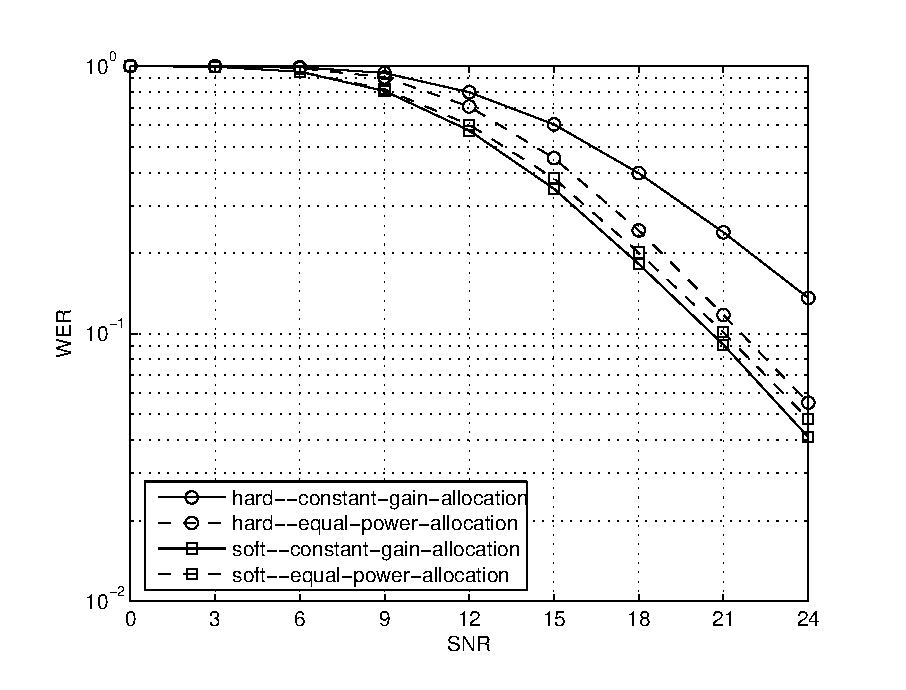
\includegraphics[width=3in]{sp_af_wer_m2_HT.eps} \label{}} \\
}
\centerline{
	\subfigure[m=3]{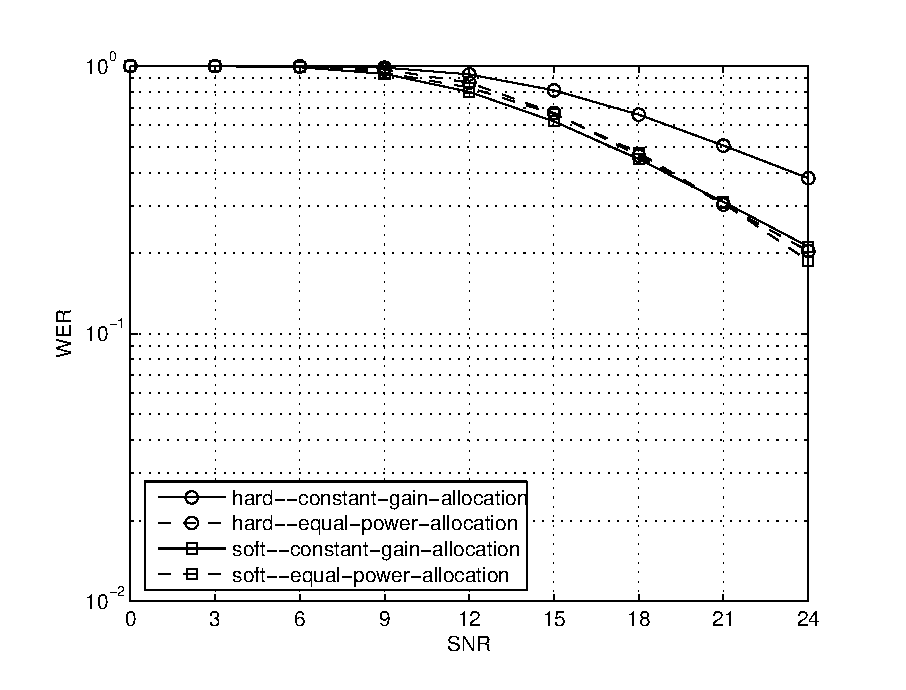
\includegraphics[width=3in]{sp_af_wer_m3_HT.eps} \label{}}
	\subfigure[m=4]{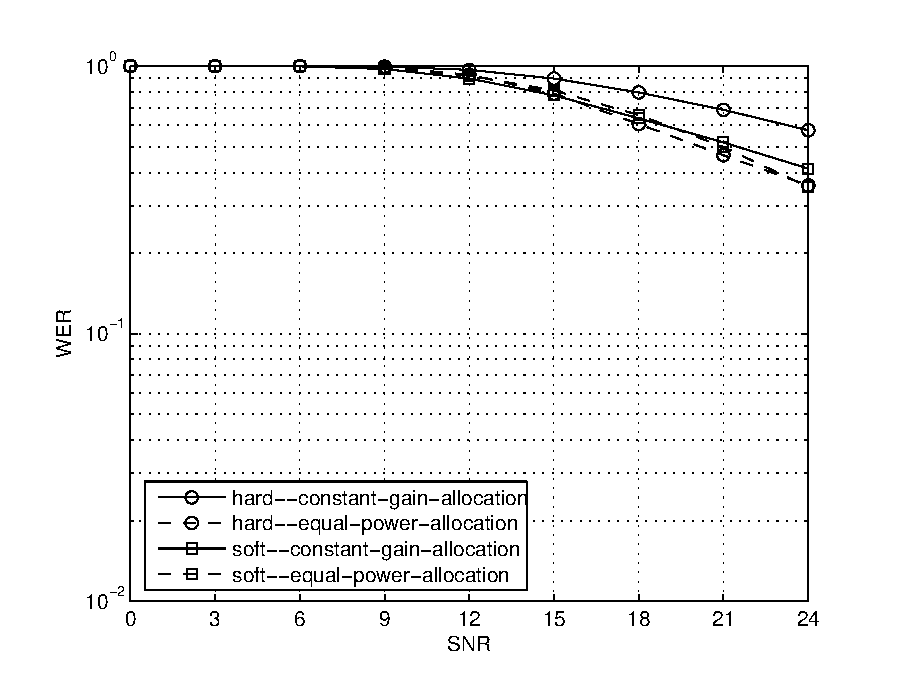
\includegraphics[width=3in]{sp_af_wer_m4_HT.eps} \label{}} \\
}
\caption{WER in a single path relay network with HT channels using AF.  $N = 128, m = 1, 2, 3$, and $4$.}
\label{fig:sp_af_wer_plots_HT}
\end{figure*}

\subsection{Decode-and-Forward}
\label{subsec:sp_bws_df}

The BER versus SNR and WER versus SNR plots for a single path relay network with TU channels using decode-and-forward are shown in Figures \ref{fig:sp_df_ber_plots_TU} and \ref{fig:sp_df_wer_plots_TU}, respectively.  The corresponding plots for HT channels are shown in Figures \ref{fig:sp_df_ber_plots_HT} and \ref{fig:sp_df_wer_plots_HT}, respectively.

As expected, soft decisions in Viterbi decoding give better performance than hard decisions.  In particular, there is up to 5 dB of SNR gain, as shown in the plots.

As we increase the distance between the transmitter and receiver (and thus, add more relays), more noise and channel distortion enter the system.  However, the error rate (BER and WER) performance suffers only slightly as $m$ increases.  TU channels and HT channels give very similar results.

\begin{figure*}
    \psfrag{BER}[Bc][tc][0.8]{BER}
    \psfrag{SNR}[tc][Bc][0.8]{SNR (dB)}
    \psfrag{hard}[cl][cl][0.5]{hard}
    \psfrag{soft}[cl][cl][0.5]{soft}

\centerline{
	\subfigure[m=1]{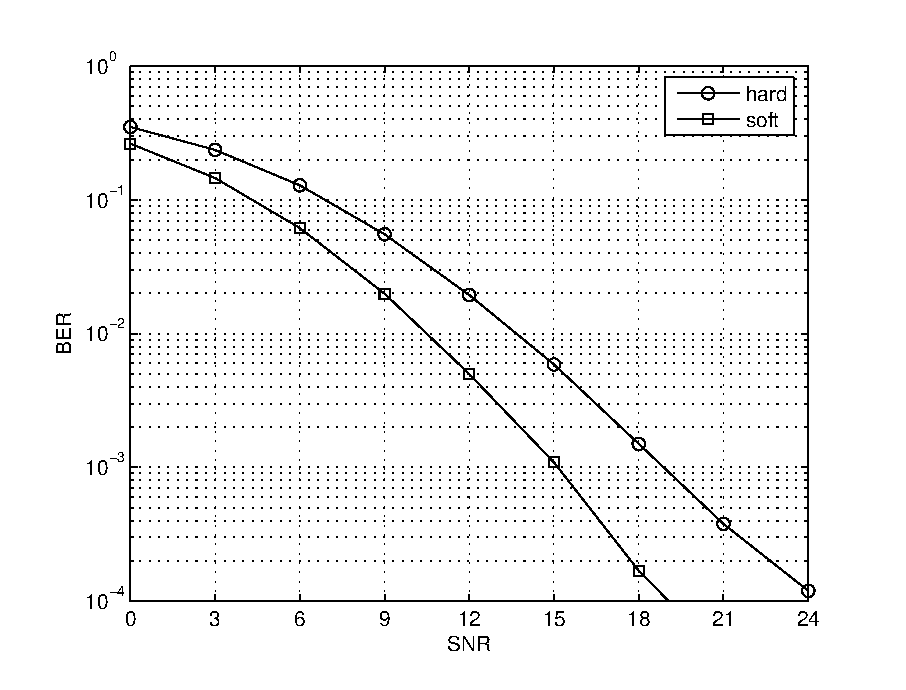
\includegraphics[width=3in]{sp_df_ber_m1_TU.eps} \label{}} 
	\subfigure[m=2]{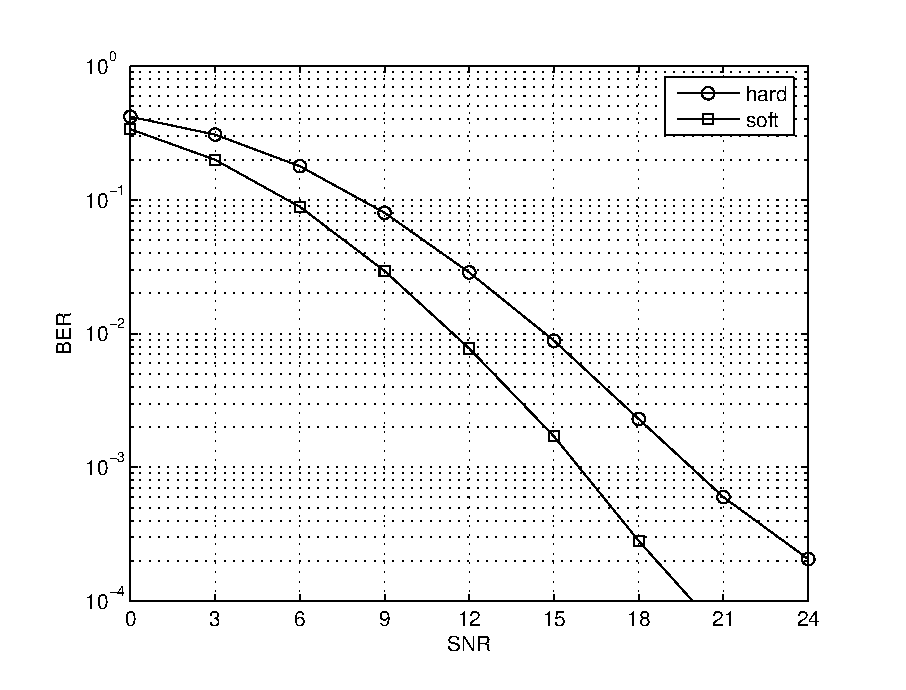
\includegraphics[width=3in]{sp_df_ber_m2_TU.eps} \label{}} \\
}
\centerline{
	\subfigure[m=3]{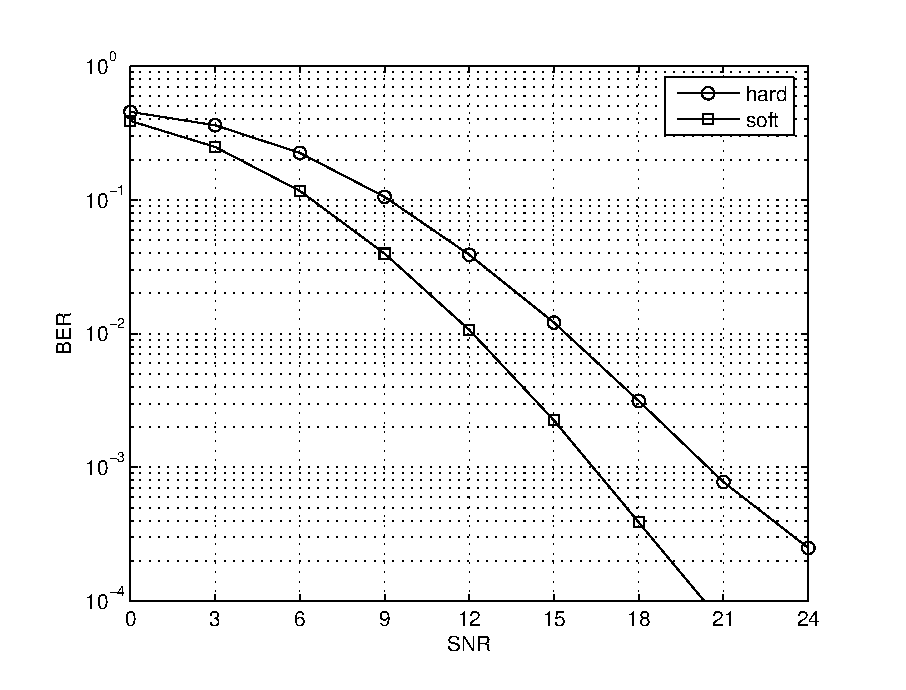
\includegraphics[width=3in]{sp_df_ber_m3_TU.eps} \label{}}
	\subfigure[m=4]{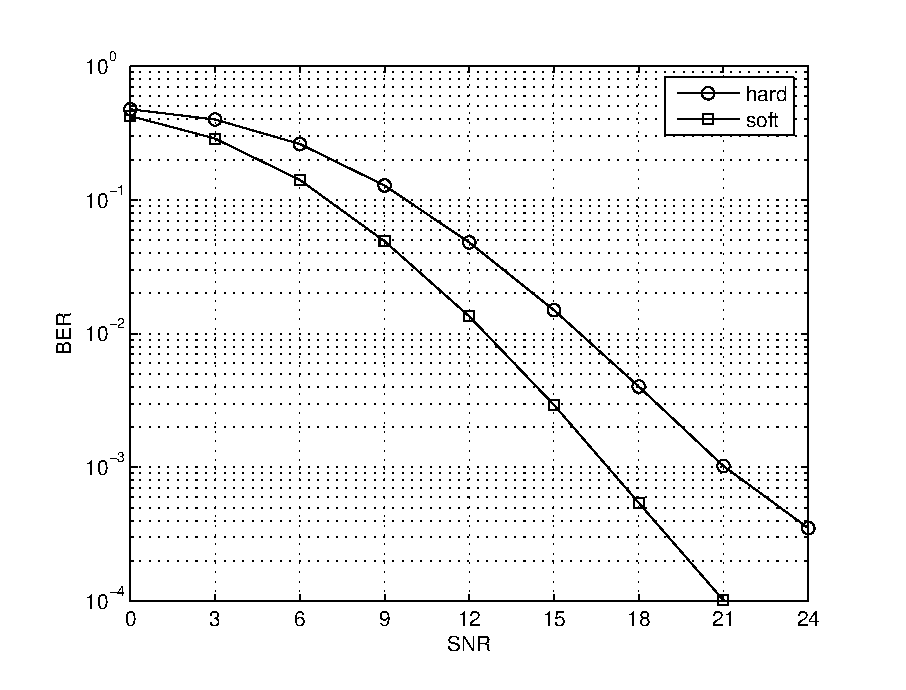
\includegraphics[width=3in]{sp_df_ber_m4_TU.eps} \label{}} \\
}
\caption{BER in a single path relay network with TU channels using DF.  $N = 128, m = 1, 2, 3$, and $4$.}
\label{fig:sp_df_ber_plots_TU}
\end{figure*}

\begin{figure*}
    \psfrag{WER}[Bc][tc][0.8]{WER}
    \psfrag{SNR}[tc][Bc][0.8]{SNR (dB)}
    \psfrag{hard}[cl][cl][0.5]{hard}
    \psfrag{soft}[cl][cl][0.5]{soft}

\centerline{
	\subfigure[m=1]{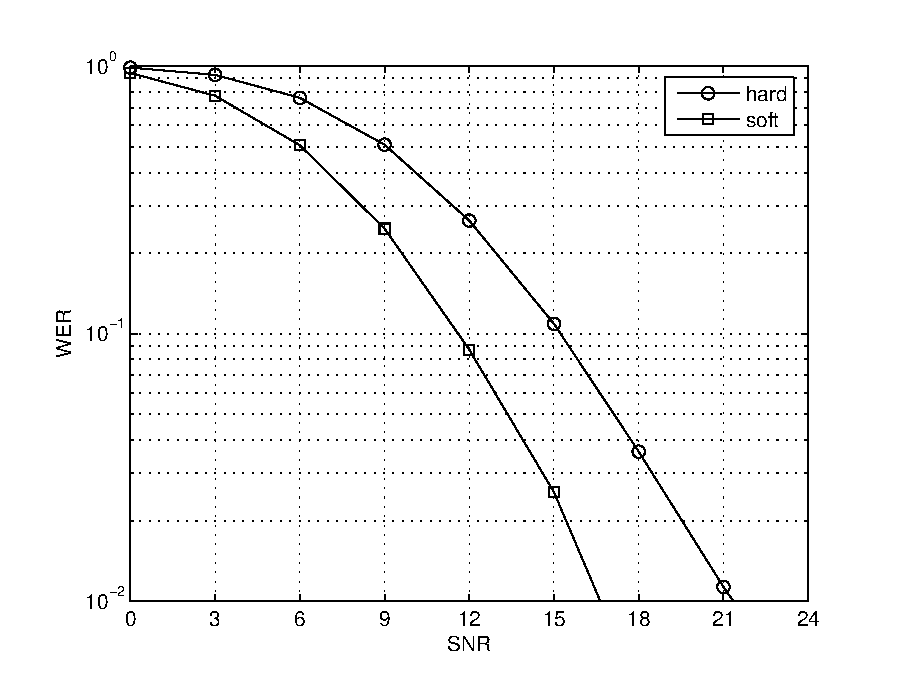
\includegraphics[width=3in]{sp_df_wer_m1_TU.eps} \label{}} 
	\subfigure[m=2]{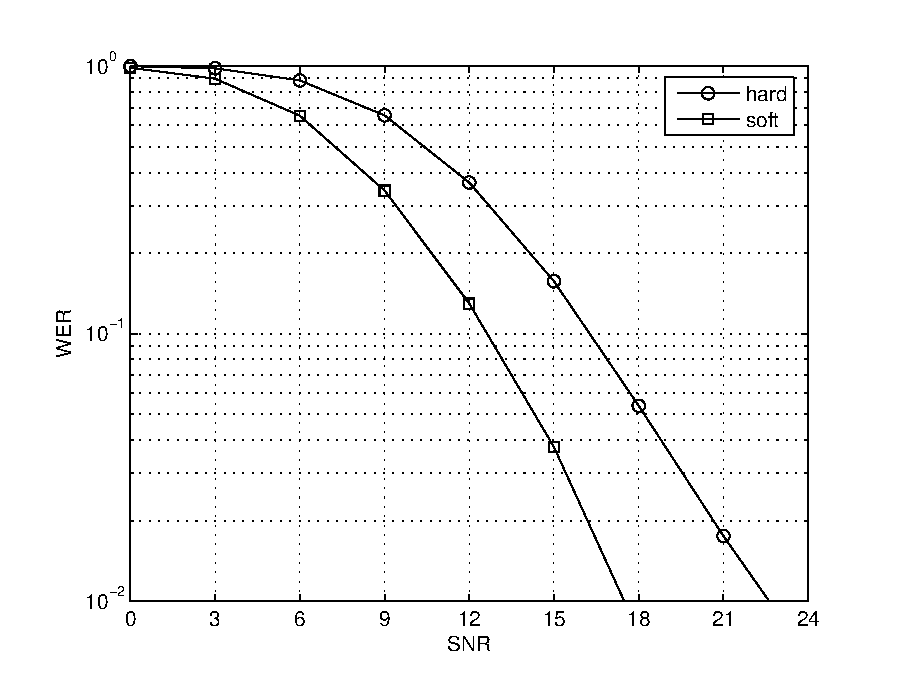
\includegraphics[width=3in]{sp_df_wer_m2_TU.eps} \label{}} \\
}
\centerline{
	\subfigure[m=3]{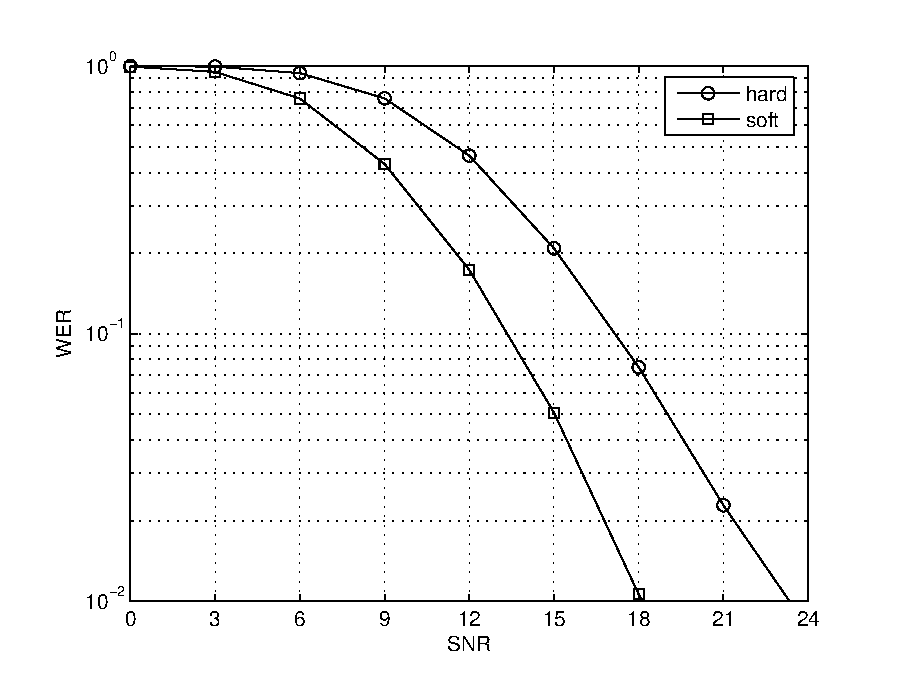
\includegraphics[width=3in]{sp_df_wer_m3_TU.eps} \label{}}
	\subfigure[m=4]{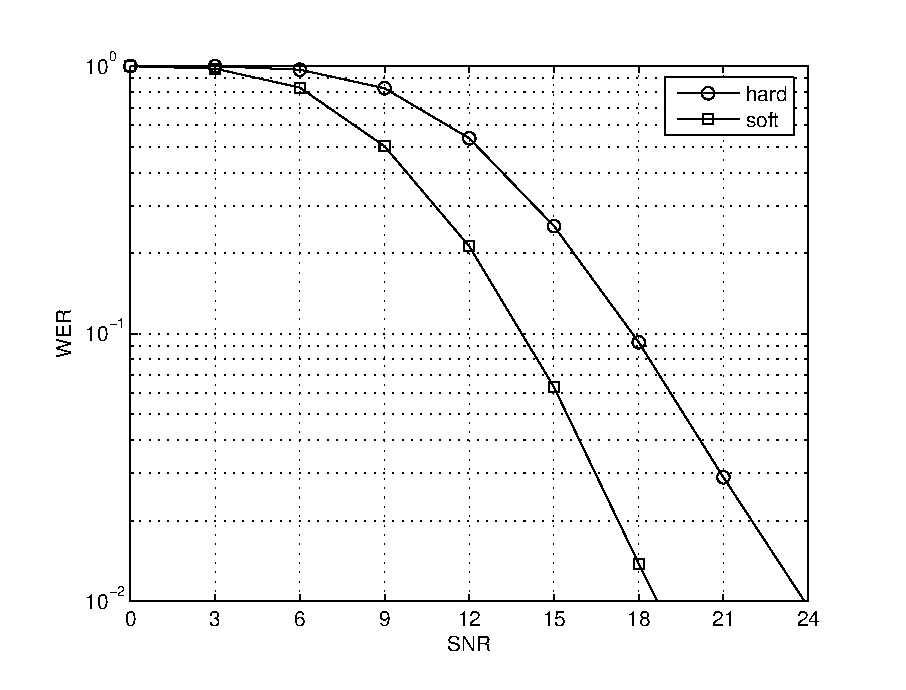
\includegraphics[width=3in]{sp_df_wer_m4_TU.eps} \label{}} \\
}
\caption{WER in a single path relay network with TU channels using DF.  $N = 128, m = 1, 2, 3$, and $4$.}
\label{fig:sp_df_wer_plots_TU}
\end{figure*}

\begin{figure*}
    \psfrag{BER}[Bc][tc][0.8]{BER}
    \psfrag{SNR}[tc][Bc][0.8]{SNR (dB)}
    \psfrag{hard}[cl][cl][0.5]{hard}
    \psfrag{soft}[cl][cl][0.5]{soft}

\centerline{
	\subfigure[m=1]{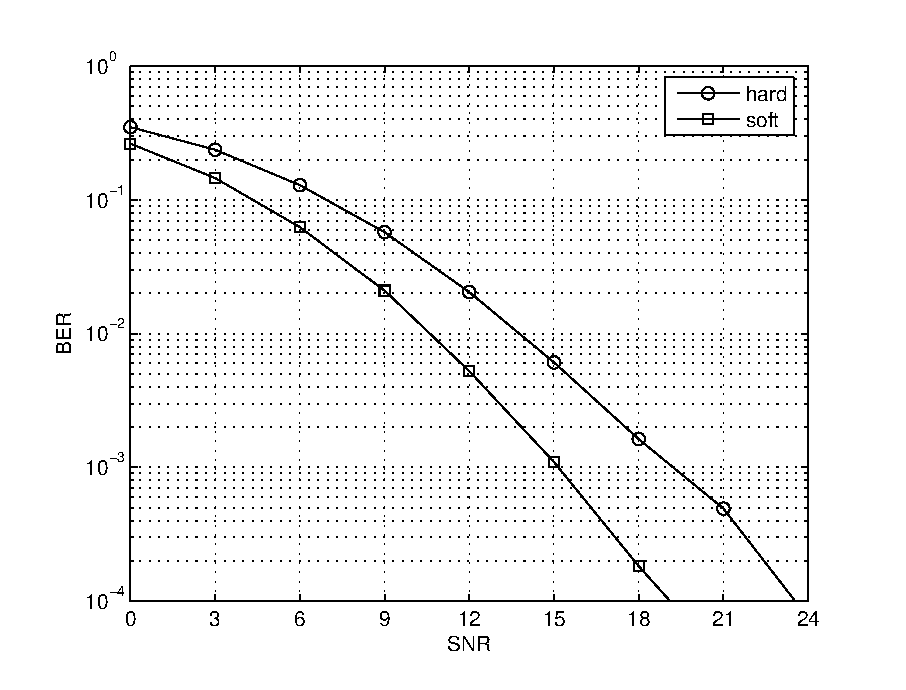
\includegraphics[width=3in]{sp_df_ber_m1_HT.eps} \label{}} 
	\subfigure[m=2]{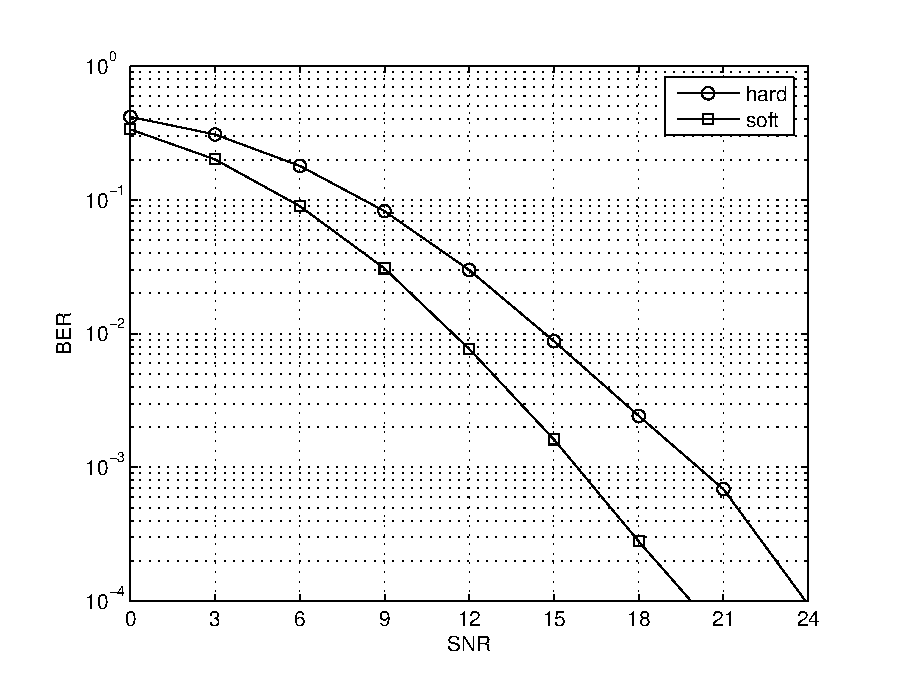
\includegraphics[width=3in]{sp_df_ber_m2_HT.eps} \label{}} \\
}
\centerline{
	\subfigure[m=3]{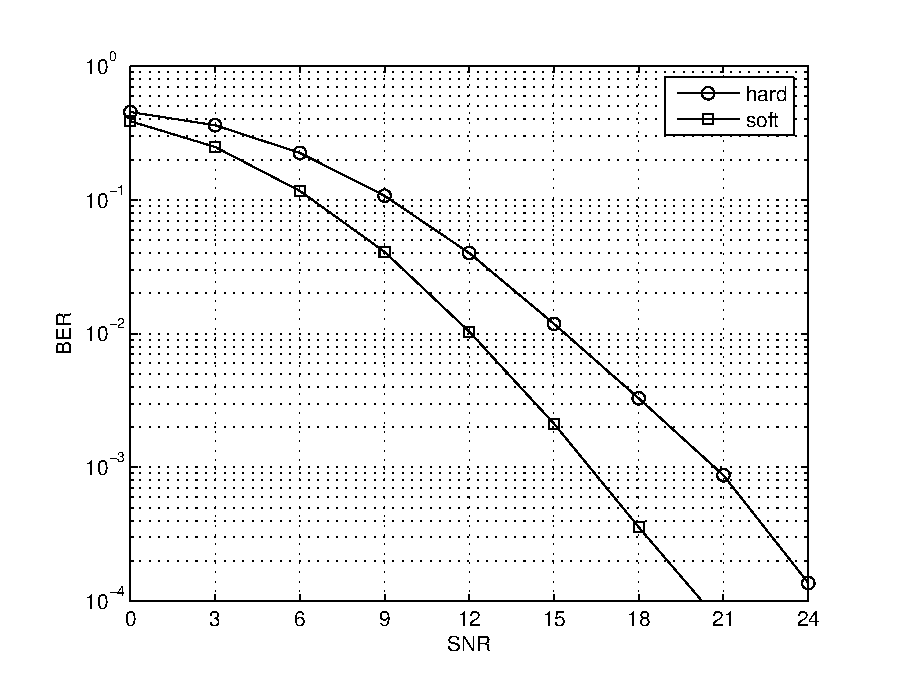
\includegraphics[width=3in]{sp_df_ber_m3_HT.eps} \label{}}
	\subfigure[m=4]{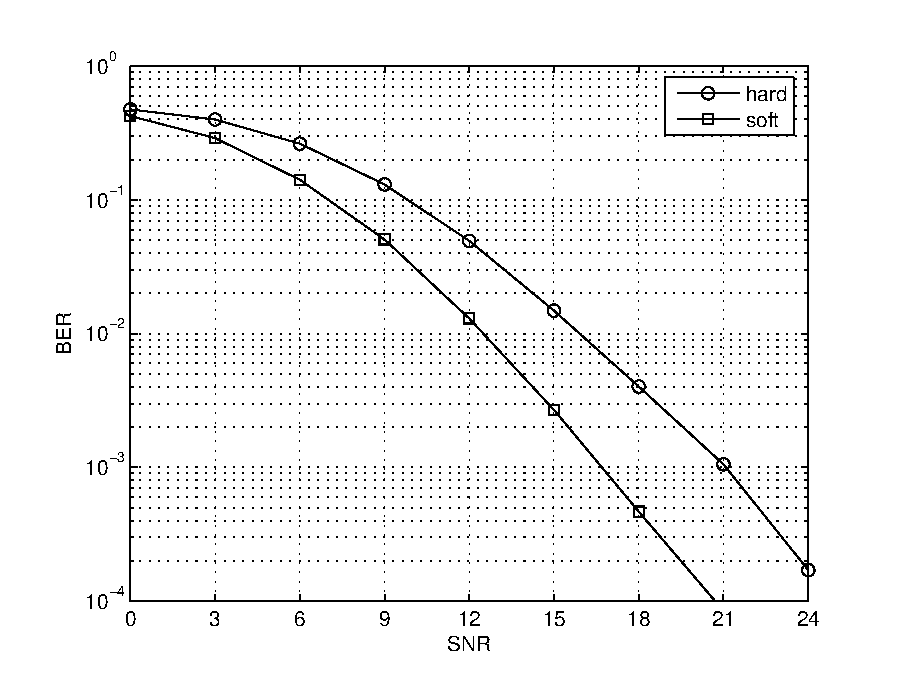
\includegraphics[width=3in]{sp_df_ber_m4_HT.eps} \label{}} \\
}
\caption{BER in a single path relay network with HT channels using DF.  $N = 128, m = 1, 2, 3$, and $4$.}
\label{fig:sp_df_ber_plots_HT}
\end{figure*}

\begin{figure*}
    \psfrag{WER}[Bc][tc][0.8]{WER}
    \psfrag{SNR}[tc][Bc][0.8]{SNR (dB)}
    \psfrag{hard}[cl][cl][0.5]{hard}
    \psfrag{soft}[cl][cl][0.5]{soft}

\centerline{
	\subfigure[m=1]{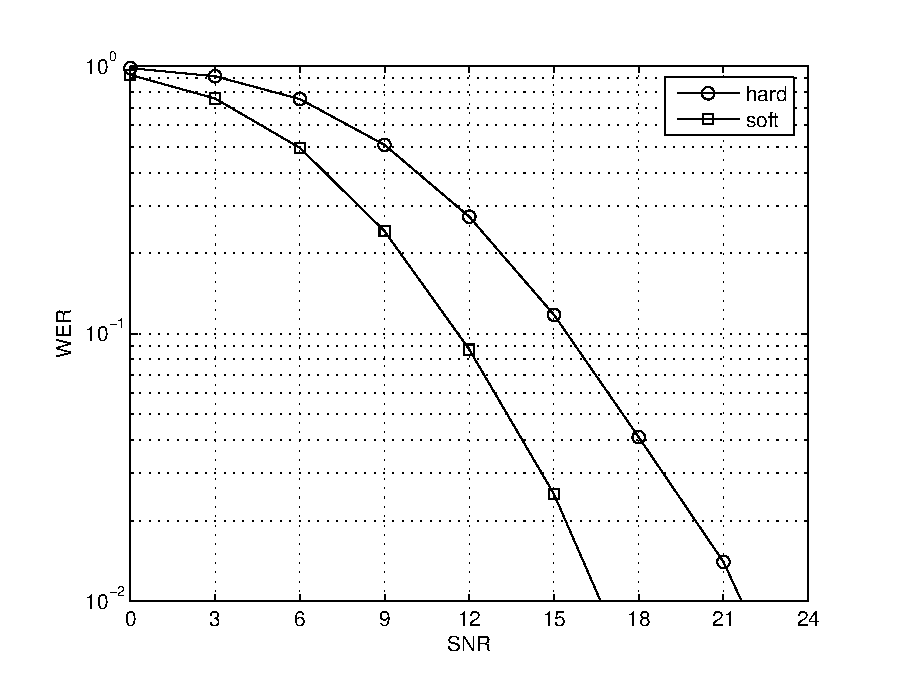
\includegraphics[width=3in]{sp_df_wer_m1_HT.eps} \label{}} 
	\subfigure[m=2]{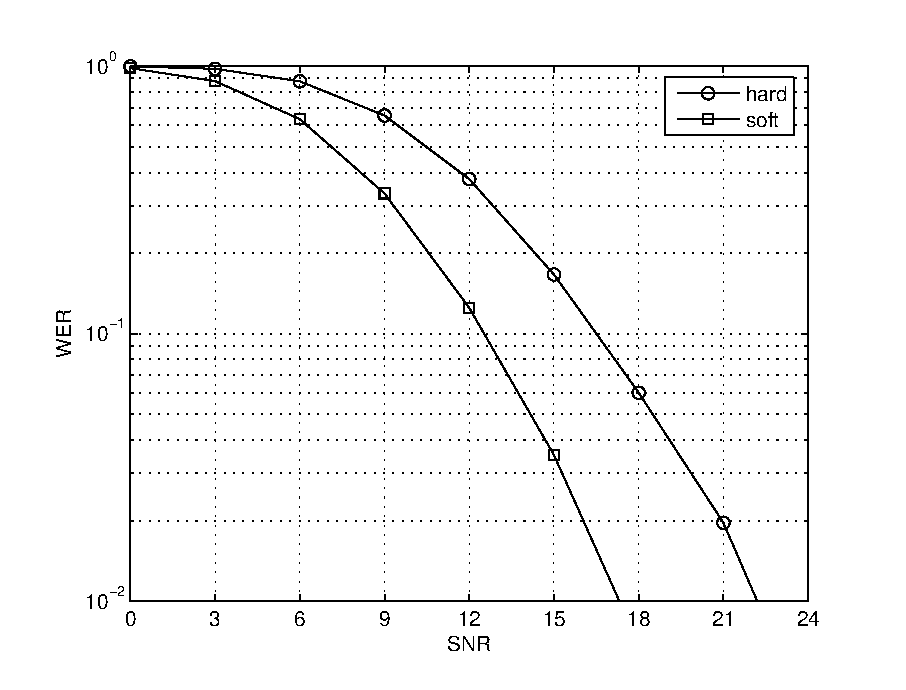
\includegraphics[width=3in]{sp_df_wer_m2_HT.eps} \label{}} \\
}
\centerline{
	\subfigure[m=3]{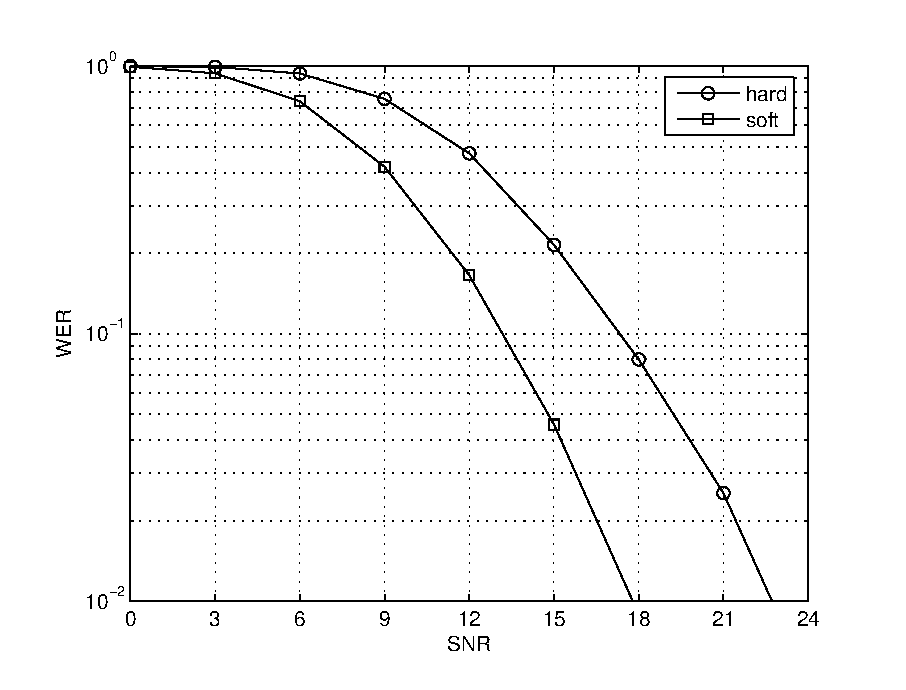
\includegraphics[width=3in]{sp_df_wer_m3_HT.eps} \label{}}
	\subfigure[m=4]{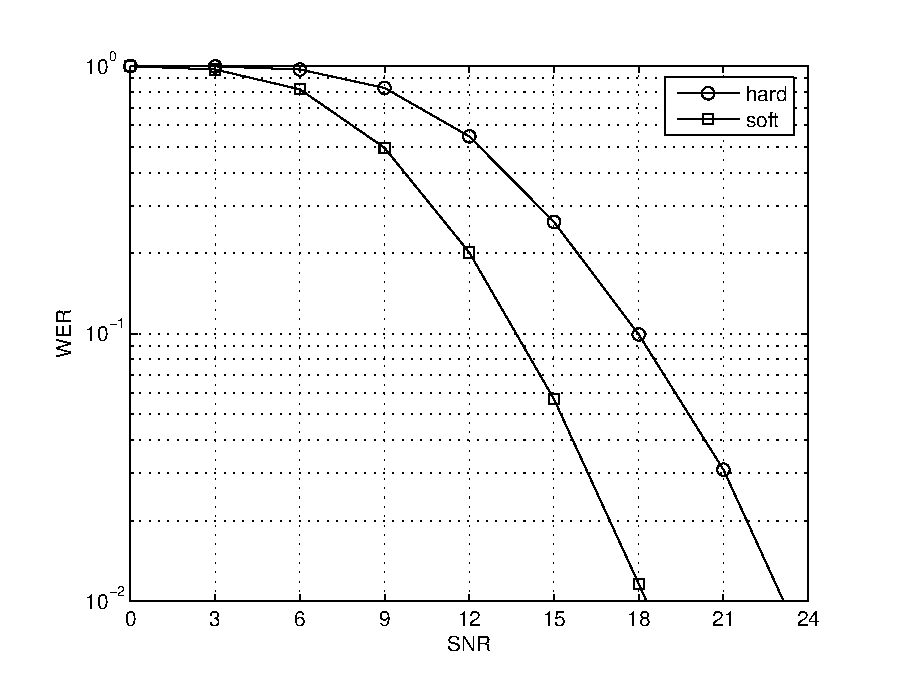
\includegraphics[width=3in]{sp_df_wer_m4_HT.eps} \label{}} \\
}
\caption{WER in a single path relay network with HT channels using DF.  $N = 128, m = 1, 2, 3$, and $4$.}
\label{fig:sp_df_wer_plots_HT}
\end{figure*}

\subsection{Comparison}
\label{subsec:sp_bws_c}

The BER versus SNR and WER versus SNR plots for a single path relay network with TU channels using amplify-and-forward and decode-and-forward are shown in Figures \ref{fig:sp_af_df_ber_plots_TU} and \ref{fig:sp_af_df_wer_plots_TU}, respectively.  The corresponding plots for HT channels are shown in Figures \ref{fig:sp_af_df_ber_plots_HT} and \ref{fig:sp_af_df_wer_plots_HT}, respectively.

As shown in the plots, there are significant error rate (BER and WER) performance gains when using decode-and-forward instead of amplify-and-forward.  The gains are even larger when we increase the distance between the transmitter and receiver (and thus, add more relays).  The amplify-and-forward error rates suffer because more noise and channel distortion enter the system.  The decode-and-forward error rates suffer only slightly because noise and channel distortion are eliminated at each relay.  This results in the large performance gains for $m=4$.

\begin{figure*}
    \psfrag{BER}[Bc][tc][0.8]{BER}
    \psfrag{SNR}[tc][Bc][0.8]{SNR (dB)}
    \psfrag{hard-af-ct----}[cl][cl][0.5]{hard, AF, CT}
    \psfrag{hard-af-eq----}[cl][cl][0.5]{hard, AF, EQ}
    \psfrag{hard-df----}[cl][cl][0.5]{hard, DF}
    \psfrag{soft-af-ct----}[cl][cl][0.5]{soft, AF, CT}
    \psfrag{soft-af-eq----}[cl][cl][0.5]{soft, AF, EQ}
    \psfrag{soft-df----}[cl][cl][0.5]{soft, DF}

\centerline{
	\subfigure[m=1]{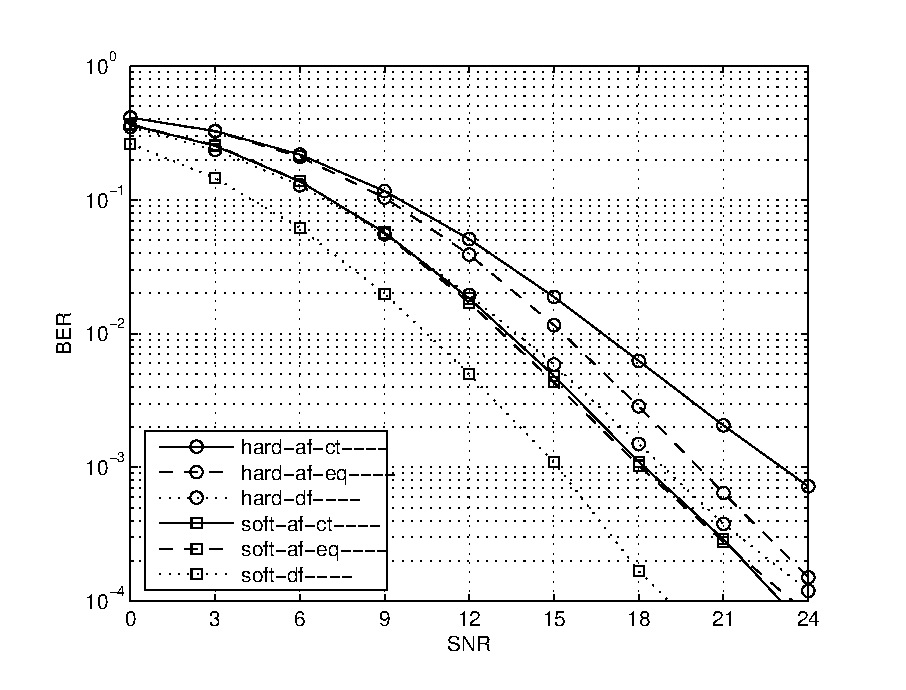
\includegraphics[width=3in]{sp_af_df_ber_m1_TU.eps} \label{}} 
	\subfigure[m=2]{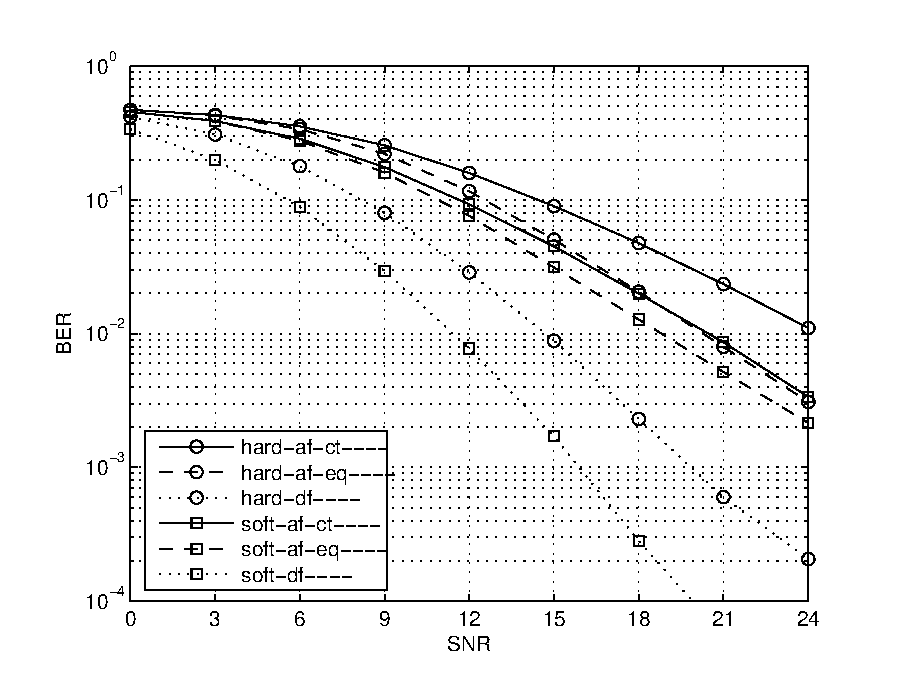
\includegraphics[width=3in]{sp_af_df_ber_m2_TU.eps} \label{}} \\
}
\centerline{
	\subfigure[m=3]{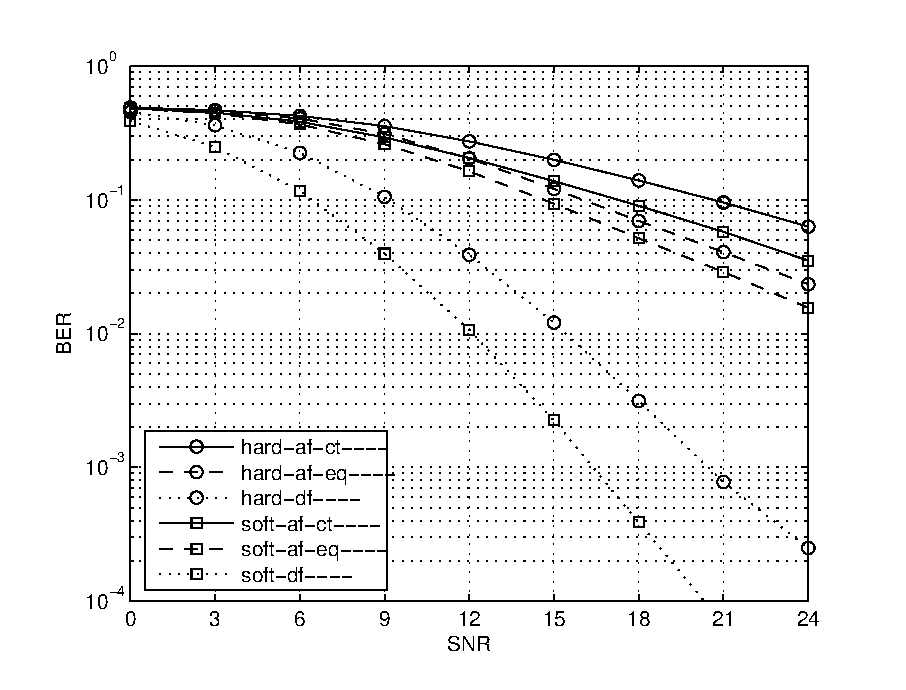
\includegraphics[width=3in]{sp_af_df_ber_m3_TU.eps} \label{}}
	\subfigure[m=4]{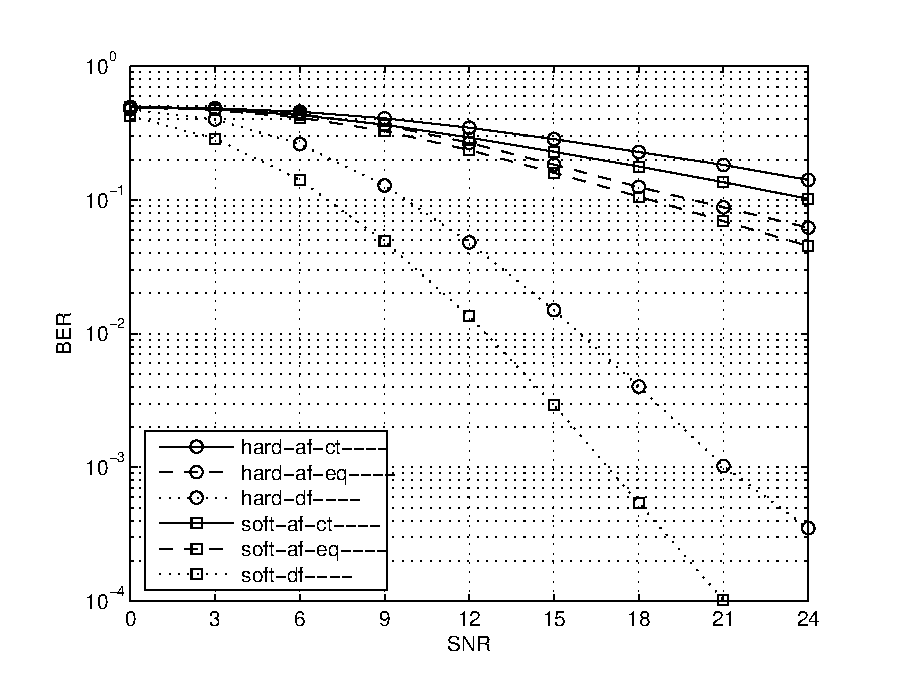
\includegraphics[width=3in]{sp_af_df_ber_m4_TU.eps} \label{}} \\
}
\caption{BER in a single path relay network with TU channels using AF and DF.  $N = 128, m = 1, 2, 3$, and $4$.}
\label{fig:sp_af_df_ber_plots_TU}
\end{figure*}

\begin{figure*}
    \psfrag{WER}[Bc][tc][0.8]{WER}
    \psfrag{SNR}[tc][Bc][0.8]{SNR (dB)}
    \psfrag{hard-af-ct----}[cl][cl][0.5]{hard, AF, CT}
    \psfrag{hard-af-eq----}[cl][cl][0.5]{hard, AF, EQ}
    \psfrag{hard-df----}[cl][cl][0.5]{hard, DF}
    \psfrag{soft-af-ct----}[cl][cl][0.5]{soft, AF, CT}
    \psfrag{soft-af-eq----}[cl][cl][0.5]{soft, AF, EQ}
    \psfrag{soft-df----}[cl][cl][0.5]{soft, DF}

\centerline{
	\subfigure[m=1]{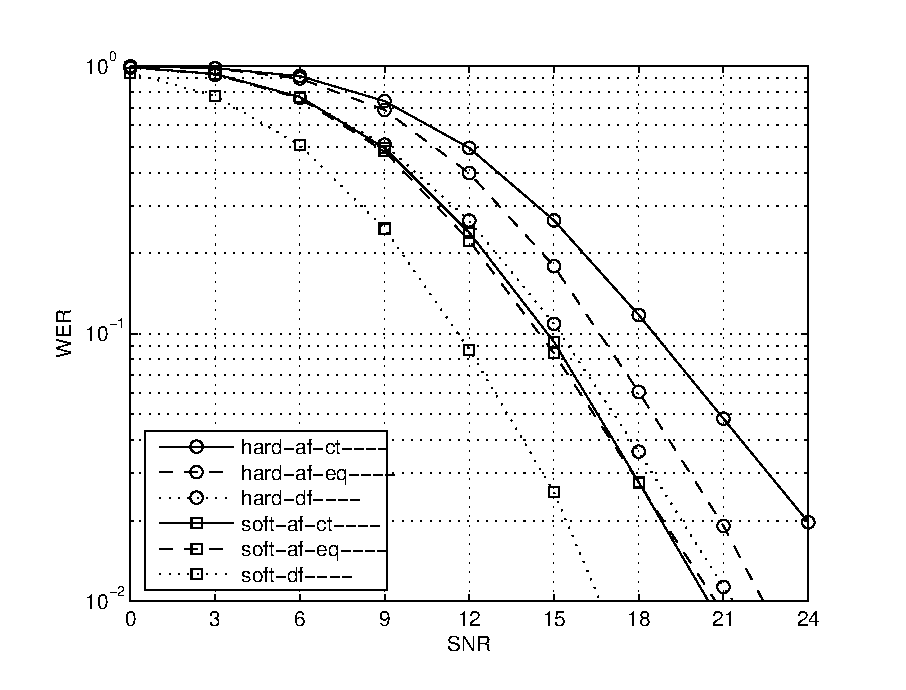
\includegraphics[width=3in]{sp_af_df_wer_m1_TU.eps} \label{}} 
	\subfigure[m=2]{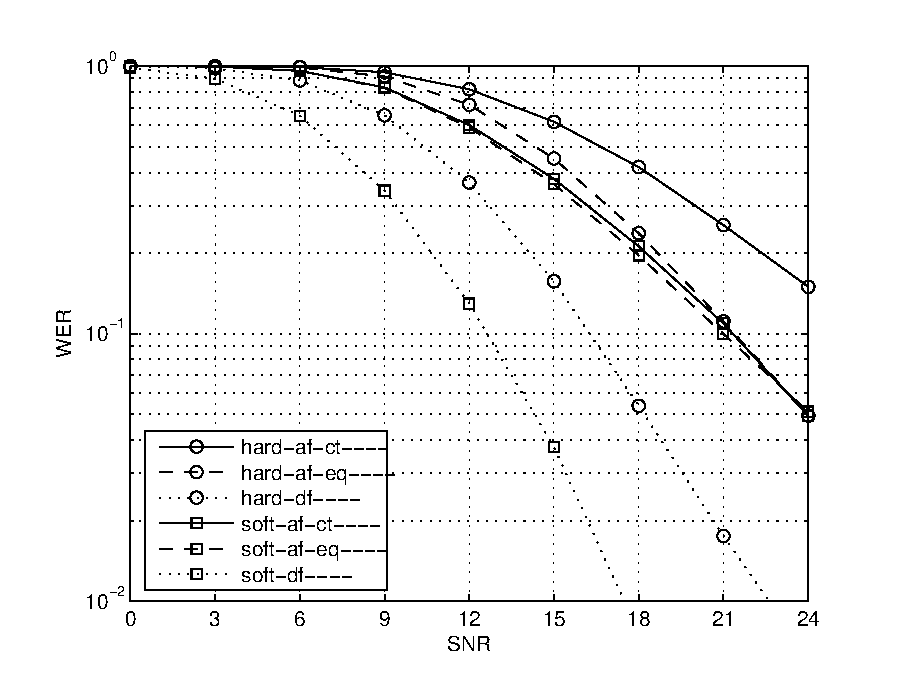
\includegraphics[width=3in]{sp_af_df_wer_m2_TU.eps} \label{}} \\
}
\centerline{
	\subfigure[m=3]{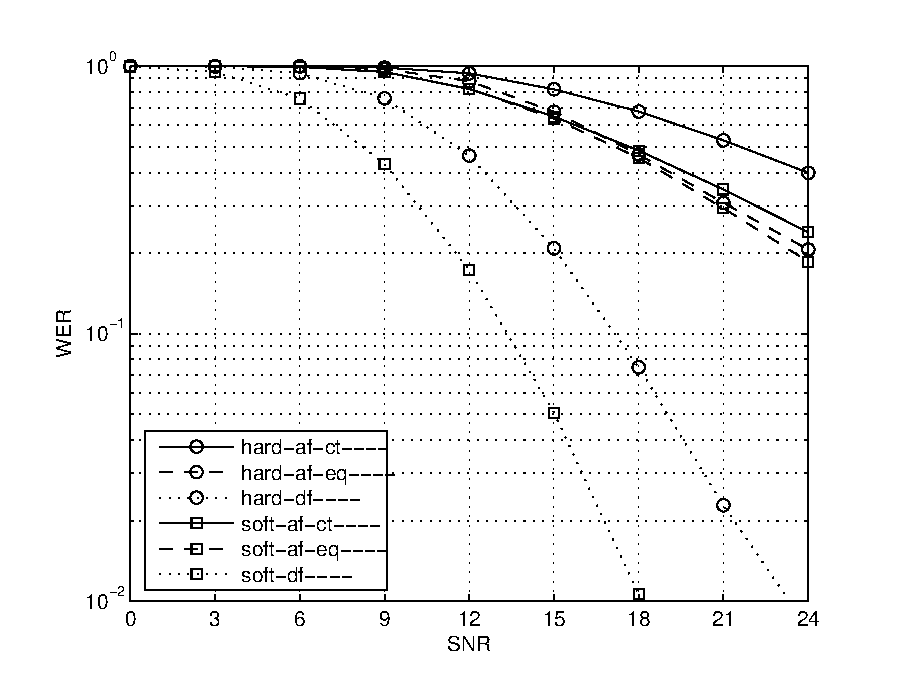
\includegraphics[width=3in]{sp_af_df_wer_m3_TU.eps} \label{}}
	\subfigure[m=4]{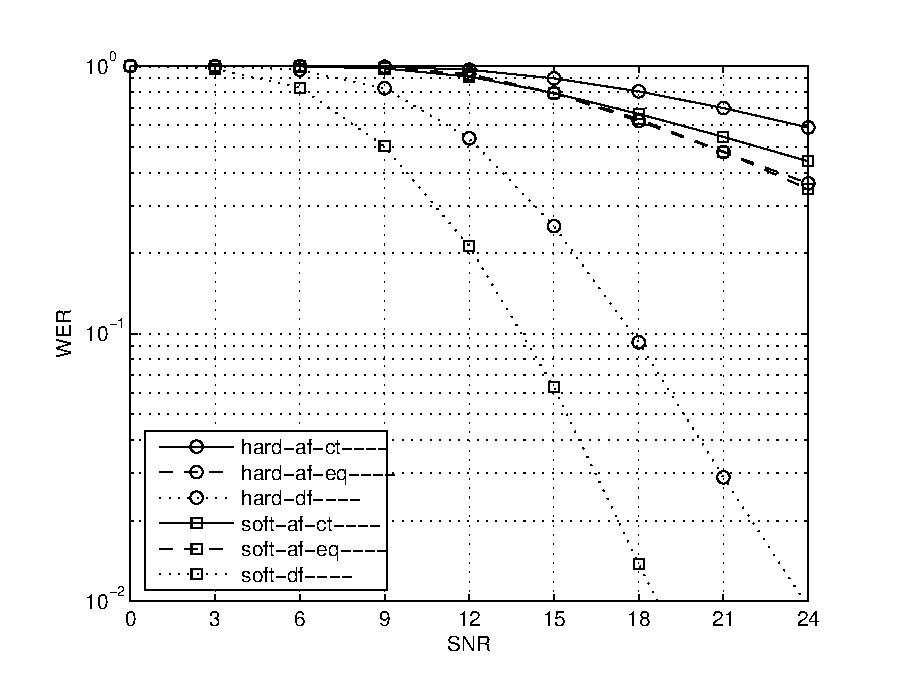
\includegraphics[width=3in]{sp_af_df_wer_m4_TU.eps} \label{}} \\
}
\caption{WER in a single path relay network with TU channels using AF and DF.  $N = 128, m = 1, 2, 3$, and $4$.}
\label{fig:sp_af_df_wer_plots_TU}
\end{figure*}

\begin{figure*}
    \psfrag{BER}[Bc][tc][0.8]{BER}
    \psfrag{SNR}[tc][Bc][0.8]{SNR (dB)}
    \psfrag{hard-af-ct----}[cl][cl][0.5]{hard, AF, CT}
    \psfrag{hard-af-eq----}[cl][cl][0.5]{hard, AF, EQ}
    \psfrag{hard-df----}[cl][cl][0.5]{hard, DF}
    \psfrag{soft-af-ct----}[cl][cl][0.5]{soft, AF, CT}
    \psfrag{soft-af-eq----}[cl][cl][0.5]{soft, AF, EQ}
    \psfrag{soft-df----}[cl][cl][0.5]{soft, DF}

\centerline{
	\subfigure[m=1]{\includegraphics[width=3in]{sp_af_df_ber_m1_HT.eps} \label{}} 
	\subfigure[m=2]{\includegraphics[width=3in]{sp_af_df_ber_m2_HT.eps} \label{}} \\
}
\centerline{
	\subfigure[m=3]{\includegraphics[width=3in]{sp_af_df_ber_m3_HT.eps} \label{}}
	\subfigure[m=4]{\includegraphics[width=3in]{sp_af_df_ber_m4_HT.eps} \label{}} \\
}
\caption{BER in a single path relay network with HT channels using AF and DF.  $N = 128, m = 1, 2, 3$, and $4$.}
\label{fig:sp_af_df_ber_plots_HT}
\end{figure*}

\begin{figure*}
    \psfrag{WER}[Bc][tc][0.8]{WER}
    \psfrag{SNR}[tc][Bc][0.8]{SNR (dB)}
    \psfrag{hard-af-ct----}[cl][cl][0.5]{hard, AF, CT}
    \psfrag{hard-af-eq----}[cl][cl][0.5]{hard, AF, EQ}
    \psfrag{hard-df----}[cl][cl][0.5]{hard, DF}
    \psfrag{soft-af-ct----}[cl][cl][0.5]{soft, AF, CT}
    \psfrag{soft-af-eq----}[cl][cl][0.5]{soft, AF, EQ}
    \psfrag{soft-df----}[cl][cl][0.5]{soft, DF}

\centerline{
	\subfigure[m=1]{\includegraphics[width=3in]{sp_af_df_wer_m1_HT.eps} \label{}} 
	\subfigure[m=2]{\includegraphics[width=3in]{sp_af_df_wer_m2_HT.eps} \label{}} \\
}
\centerline{
	\subfigure[m=3]{\includegraphics[width=3in]{sp_af_df_wer_m3_HT.eps} \label{}}
	\subfigure[m=4]{\includegraphics[width=3in]{sp_af_df_wer_m4_HT.eps} \label{}} \\
}
\caption{WER in a single path relay network with HT channels using AF and DF.  $N = 128, m = 1, 2, 3$, and $4$.}
\label{fig:sp_af_df_wer_plots_HT}
\end{figure*}

\chapter{Multiple Path Relay Network}
\label{chap:mp}

\begin{figure}
  \centering
    \psfrag{r0}[cc][Bl][0.9]{$r_0$}
    \psfrag{r1}[cc][Bl][0.9]{$r_1$}
    \psfrag{r3}[cc][Bl][0.9]{$r_m$}
    \psfrag{r4}[cc][Bl][0.9]{$r_{m+1}$}
    \psfrag{n01}[cc][Bl][0.8]{$n_k^{(0|1)}$}
    \psfrag{n03}[cc][Bl][0.8]{$n_k^{(0|m)}$}
    \psfrag{n14}[cc][Bl][0.8]{$n_k^{(1|m+1)}$}
    \psfrag{n34}[cc][Bl][0.8]{$n_k^{(m|m+1)}$}
    \psfrag{H01}[cc][Bl][0.8]{$h_k^{(0|1)}$}
    \psfrag{H03}[cc][Bl][0.8]{$h_k^{(0|m)}$}
    \psfrag{H14}[cc][Bl][0.8]{$h_k^{(1|m+1)}$}
    \psfrag{H34}[cc][Bl][0.8]{$h_k^{(m|m+1)}$}
    \psfrag{Tx}[cr][Bl][0.9]{Transmitter}
    \psfrag{Rx}[cl][Bl][0.9]{Receiver}
    \includegraphics[width=5in]{mp_model.eps}
   \caption{Multiple Path Relay Network \label{fig:mp_sm} }
\end{figure}

\section{Amplify-and-Forward}
\label{sec:mp_af}

\subsection{System Model}
\label{subsec:mp_af_sm}

Figure \ref{fig:mp_sm} shows the multiple path relay network.  In the figure, $r_0$ is the transmitter, $r_{m+1}$ is the receiver, and $r_1, \ldots, r_m$ are $m$ relay nodes connected in parallel forming a multiple path link between the transmitter and receiver.  The relays perform amplify-and-forward (AF) relaying.  We assume that OFDM with $N$ subcarriers is used in the system.

$h_k^{(0|1)}, \ldots, h_k^{(0|m)}, h_k^{(1|m+1)}, \ldots, h_k^{(m|m+1)}$ are the complex subchannel gains at the $k^{\mbox{th}}$ subcarrier in the link, for $k = 1$ to $N$.   $n_k^{(0|1)}, \ldots, n_k^{(0|m)}, n_k^{(1|m+1)}, \ldots, n_k^{(m|m+1)}$ are the corresponding noises, which are assumed to be mutually independent, zero-mean, circular symmetric complex Gaussians all with variance $N_0 B / N$, where $N_0$ is the power spectral density of the underlying continuous time noise process and $B$ is the OFDM bandwidth of the system.  Let $p_k^{(0)} = P_{\mbox{tot}}/N$ be the transmitter power on the $k^{\mbox{th}}$ subcarrier, where $P_{\mbox{tot}}$ is the net transmitter power.  Let  $\sqrt{p_k^{(l)}}$ be the amplifying gain used in the amplify-and-forward algorithm at the $l^{\mbox{th}}$ relay, for $l=1$ to $m$.  The $k^{\mbox{th}}$ receive symbol at $r_l$ is amplified by $\sqrt{p_k^{(l)}}$ before it is forwarded to the next node.

Let $x_k$ be the $k^{\mbox{th}}$ transmit symbol with zero mean and unit variance.  Let $y_k^{(l)}$  be the $k^{\mbox{th}}$ receive symbol from the $l^{\mbox{th}}$ path at the receiver.  Using Figure \ref{fig:mp_sm}, the input-output relation for the $l^{\mbox{th}}$ path is
\begin{eqnarray}
y_k^{(l)} = \left( h_k^{(0|l)} h_k^{(l|m+1)} \sqrt{p_k^{(0)}} \sqrt{p_k^{(l)}} \right) x_k
+\left( h_k^{(l|m+1)} \sqrt{p_k^{(l)}} \right) n_k^{(0|l)} +  n_k^{(l|m+1)}.
\label{eqn:mp_af_inout}
\end{eqnarray}
If we define
\begin{eqnarray}
\mathbf{y}_k = \left[
\begin{array}{ccc}
y_k^{(1)} &
\cdots &
y_k^{(m)} 
\end{array} \right]^T,
\end{eqnarray}
\begin{eqnarray}
\mathbf{h}_k = \left[
\begin{array}{ccc}
h_k^{(0|1)}h_k^{(1|m+1)} \sqrt{p_k^{(0)}} \sqrt{p_k^{(1)}} & \cdots & h_k^{(0|m)}h_k^{(m|m+1)} \sqrt{p_k^{(0)}} \sqrt{p_k^{(m)}}
\end{array}
\right]^T,
\label{eqn:mp_af_hk}
\end{eqnarray}
\begin{eqnarray}
\mathbf{\Gamma}_k = \left[
\begin{array}{cccccccc}
h_k^{(1|m+1)} \sqrt{p_k^{(1)}}&  & \textbf{\mbox{\huge{0}}} & 1 & & & & \textbf{\mbox{\huge{0}}}  \\
 & \ddots & & & & \ddots & &  \\
\textbf{\mbox{\huge{0}}} &  &h_k^{(m|m+1)} \sqrt{p_k^{(m)}} & \textbf{\mbox{\huge{0}}} & & & & 1 
\end{array}
\right]
\mbox{,}
\label{eqn:mp_af_Gammak}
\end{eqnarray}
\begin{eqnarray}
\mathbf{n}_k = \left[
\begin{array}{cccccc}
n_k^{(0|1)} & \cdots & n_k^{(0|m)} & n_k^{(1|m+1)} & \cdots & n_k^{(m|m+1)}
\end{array} \right]^T\mbox{,}
\label{eqn:mp_af_nk}
\end{eqnarray}
and
\begin{eqnarray}
\mathbf{w}_k = \mathbf{\Gamma}_k \mathbf{n}_k \mbox{,} 
\label{eqn:mp_af_wk}
\end{eqnarray}
then (\ref{eqn:mp_af_inout}), for all $l = 1$ to $m$, can be written as
\begin{eqnarray}
\mathbf{y}_k = \mathbf{h}_k x_k + \mathbf{w}_k \mbox{.}
\label{eqn:mp_af_inout_terse}
\end{eqnarray}
The large boldface zeros in (\ref{eqn:mp_af_Gammak}) represent zero values in the off diagonal entries in the two $m \times m$ submatrices of $\mathbf{\Gamma}_k$.  

Now, consider the covariance of $\mathbf{w}_k$.  Using (\ref{eqn:mp_af_Gammak}), (\ref{eqn:mp_af_nk}), and (\ref{eqn:mp_af_wk}), we have
\begin{eqnarray}
R_{\mathbf{w}_k\mathbf{w}_k} & = & E \left[ \mathbf{w}_k \mathbf{w}_k^H \right] \\
& = & E \left[ \mathbf{\Gamma}_k \mathbf{n}_k \mathbf{n}_k^H \mathbf{\Gamma}_k^H \right] \\
& = & \mathbf{\Gamma}_k E \left[ \mathbf{n}_k \mathbf{n}_k^H  \right] \mathbf{\Gamma}_k^H \\
& = &  \frac{N_0B}{N} \left[
\begin{array}{ccc}
b_k^{(1|m+1)} p_k^{(1)}  + 1 & & \textbf{\mbox{\huge{0}}} \\
 & \ddots & \\
\textbf{\mbox{\huge{0}}}  & &  b_k^{(m|m+1)} p_k^{(m)} + 1
\end{array} \right],
\label{eqn:mp_af_Rwkwk}
\end{eqnarray}
where $E\left[ \cdot \right]$ is the expectation operator, $\left( \cdot \right)^H$ is the Hermitian (complex transpose) operator for a vector or matrix, and $b_k^{(i|j)} = \left| h_k^{(i|j)} \right|^2$, for $i=0$ to $m$, for $j=1$ to $m+1$, and $i \neq j$.  Since the diagonal entries of $R_{\mathbf{w}_k\mathbf{w}_k}$ are never zero, $R_{\mathbf{w}_k\mathbf{w}_k}^{-1}$ and $R_{\mathbf{w}_k\mathbf{w}_k}^{-\frac{1}{2}}$ are well defined, where $R_{\mathbf{w}_k\mathbf{w}_k}^{-\frac{1}{2}}R_{\mathbf{w}_k\mathbf{w}_k}^{-\frac{1}{2}} = R_{\mathbf{w}_k\mathbf{w}_k}^{-1}$
\begin{eqnarray}
R_{\mathbf{w}_k\mathbf{w}_k}^{-1} = \frac{N}{N_0B} \left[
\begin{array}{ccc}
\frac{1}{ b_k^{(1|m+1)} p_k^{(1)}+ 1} & & \textbf{\mbox{\huge{0}}} \\
 & \ddots & \\
\textbf{\mbox{\huge{0}}}  & & \frac{1}{ b_k^{(m|m+1)}p_k^{(m)} + 1}
.\label{eqn:mp_af_Rwkwk_inv}
\end{array} \right]. 
\end{eqnarray}
Also, if we define $R_{\mathbf{w}_k\mathbf{w}_k}$ as $R_{\mathbf{w}_k\mathbf{w}_k}^{\frac{1}{2}} R_{\mathbf{w}_k\mathbf{w}_k}^{\frac{1}{2}} =R_{\mathbf{w}_k\mathbf{w}_k}$, then $R_{\mathbf{w}_k\mathbf{w}_k}^{-\frac{1}{2}}R_{\mathbf{w}_k\mathbf{w}_k}^{\frac{1}{2}} = R_{\mathbf{w}_k\mathbf{w}_k}^{\frac{1}{2}}R_{\mathbf{w}_k\mathbf{w}_k}^{-\frac{1}{2}} = \mathbf{I}$.
We define a transformed version of the system in (\ref{eqn:mp_af_inout_terse})
\begin{eqnarray}
\tilde{\mathbf{y}}_k = \tilde{\mathbf{h}}_k x_k + \tilde{\mathbf{w}}_k,
\end{eqnarray}
where $\tilde{\mathbf{y}}_k = R_{\mathbf{w}_k\mathbf{w}_k}^{-\frac{1}{2}} \mathbf{y}_k$, $\tilde{\mathbf{h}}_k =R_{\mathbf{w}_k\mathbf{w}_k}^{-\frac{1}{2}} \mathbf{h}_k$, and $\tilde{\mathbf{w}}_k = R_{\mathbf{w}_k\mathbf{w}_k}^{-\frac{1}{2}} \mathbf{w}_k$.  The covariance matrices of $\tilde{\mathbf{w}}_k$ and $\tilde{\mathbf{y}}_k$ are
\begin{eqnarray}
E \left[ \tilde{\mathbf{w}}_k \tilde{\mathbf{w}}_k^H \right] & = & E \left[R_{\mathbf{w}_k\mathbf{w}_k}^{-\frac{1}{2}} \mathbf{w}_k \mathbf{w}_k^H R_{\mathbf{w}_k\mathbf{w}_k}^{-\frac{1}{2}} \right] \\
& = & R_{\mathbf{w}_k\mathbf{w}_k}^{-\frac{1}{2}} R_{\mathbf{w}_k\mathbf{w}_k}R_{\mathbf{w}_k\mathbf{w}_k}^{-\frac{1}{2}} \\
& = & \mathbf{I} 
\end{eqnarray}
and
\begin{eqnarray}
E \left[ \tilde{\mathbf{y}}_k \tilde{\mathbf{y}}_k^H \right] & = & E \left[ \left(\tilde{\mathbf{h}_k}x_k + \tilde{\mathbf{w}_k}\right) \left(\tilde{\mathbf{h}_k}x_k + \tilde{\mathbf{w}_k}\right)^H \right] 
\\
& = & \tilde{\mathbf{h}}_k \tilde{\mathbf{h}}_k^H + \mathbf{I},
\label{eqn:mp_af_yk_tilde_covar}
\end{eqnarray}
respectively.  The cross terms do not appear in (\ref{eqn:mp_af_yk_tilde_covar}) because $\tilde{\mathbf{h}_k}$, $\tilde{\mathbf{w}_k}$ and $x_k$ are mutually independent.  Note that the transformed system has identity covariance noise.

\subsection{Mutual Information}
\label{subsec:mp_af_mi}

To derive the mutual information, note that the differential entropy of a circular symmetric complex Gaussian vector, $\mathbf{v}$, with covariance matrix, $\mathbf{K}$, is $h\left(\mathbf{v}\right) = \log_2 \det \left( \pi e \mathbf{K} \right)$ \cite{article:Telatar01}.  Let $\mathcal{I}_k$ be the mutual information between the transmitter and receiver on the $k^{\mbox{th}}$ subcarrier
\begin{eqnarray}
\mathcal{I}_k & = & h\left( \tilde{\mathbf{y}}_k \right) - h \left( \tilde{\mathbf{w}}_k \right)  \\
& = & \log_2 \det\left[ \pi e \left(\tilde{\mathbf{h}}_k \tilde{\mathbf{h}}_k^H + \mathbf{I} \right) \right] 
- \log_2 \det \left( \pi e \mathbf{I} \right)  \\
& = & \log_2 \left( 1 + \mathbf{h}_k^H R_{\mathbf{w}_k\mathbf{w}_k}^{-1} \mathbf{h}_k \right),
\label{eqn:mp_af_Ik}
\end{eqnarray}
where the first equality comes from basic mutual information calculations \cite{book:Cover01}.  The third equality follows from the properties of determinants of matrices.  The total mutual information between the transmitter and receiver, $\mathcal{I}$, is the sum of all $\mathcal{I}_k$ divided by $N$.  That is, after substituting (\ref{eqn:mp_af_hk}) and (\ref{eqn:mp_af_Rwkwk_inv}) into (\ref{eqn:mp_af_Ik}), we have
\begin{eqnarray}
\mathcal{I} & = & \frac{1}{N}  \sum_{k=1}^N \mathcal{I}_k \\
& = & \frac{1}{N}  \sum_{k=1}^N \log_2 \left[ 1 + \mbox{SNR} \sum_{i=1}^m \left(
\frac{b_k^{(0|i)} b_k^{(i|m+1)}p_k^{(i)}  }{ b_k^{(i|m+1)} p_k^{(i)}+1 }\right) \right],
\label{eqn:mp_af_I}
\end{eqnarray}
where $\mbox{SNR} = P_{\mbox{tot}}/N_0B$.  If we denote	
\begin{eqnarray}
\mathbf{B}^{(\mbox{sr})} = \left[ \begin{array}{ccc}
b_1^{(0|1)} & \cdots & b_1^{(0|m)} \\
\vdots & \ddots & \vdots \\
b_N^{(0|1)} & \cdots & b_N^{(0|m)}
\end{array}
\right] \mbox{,} &
\mathbf{B}^{(\mbox{rd})} = \left[ \begin{array}{ccc}
b_1^{(1|m+1)} & \cdots & b_1^{(m|m+1)} \\
\vdots & \ddots & \vdots \\
b_N^{(1|m+1)} & \cdots & b_N^{(m|m+1)}
\end{array}
\right] \mbox{,}
\label{}
\end{eqnarray}
\begin{eqnarray}
 & \mathbf{P} = \left[ \begin{array}{ccc}
p_1^{(1)} & \cdots & p_1^{(m)} \\
\vdots & \ddots & \vdots \\
p_N^{(1)} & \cdots & p_N^{(m)}
\end{array}
\right] \mbox{,}
\label{}
\end{eqnarray}
\begin{eqnarray}
\begin{array}{ccc}
\mathbf{e}_N = \underbrace{\left[ \begin{array}{ccc}
1 & \cdots & 1
\end{array}
\right]^T}_{\mbox{$N$ ones}} \mbox{,}& \mbox{and} &
\mathbf{e}_m = \underbrace{\left[ \begin{array}{ccc}
1 & \cdots & 1
\end{array}
\right]^T}_{\mbox{$m$ ones}},
\end{array}
\label{}
\end{eqnarray}
then (\ref{eqn:mp_af_I}) can be written in matrix form.  First, let
\begin{eqnarray}
\mathbf{z}_{\mbox{multiple}} = 
\left[ \left( \mathbf{B}^{(\mbox{sr})} \circ \mathbf{B}^{(\mbox{rd})} \circ \mathbf{P}  \right) \circ / \left( \mathbf{B}^{(\mbox{rd})} \circ \mathbf{P}  + \mathbf{e}_N \mathbf{e}_m^T \right) \right] \mathbf{e}_m,
\end{eqnarray}
where the $\circ$ and $\circ /$ operators represent element-wise matrix multiplication and element-wise matrix division, respectively.  Then, (\ref{eqn:mp_af_I}) in matrix form is
\begin{eqnarray}
\mathcal{I} = \frac{1}{N} \mathbf{e}_N^T \log_2 \left( \mathbf{e}_N + \mbox{SNR} \: \mathbf{z}_{\mbox{multiple}} \right) ,
\label{eqn:mp_af_I_matrix}
\end{eqnarray}
where $\log_2\left( \cdot \right)$ of a vector is the vector of the logarithms of the vector's entries.

\subsection{Relay Power Allocation}
\label{subsec:mp_af_rpa}

We assume that the net transmit power at the transmitter and at each each relay is $P_{\mbox{tot}}$.  At the transmitter, we assume a uniform power distribution, that is, $p_k^{(0)} = P_{\mbox{tot}}/N$.  To derive the power constraint at each relay and thus, possible power allocations, consider $v_k^{(l)}$, the $k^{\mbox{th}}$ transmit symbol of $r_l$
\begin{eqnarray}
v_k^{(l)} = \sqrt{p_k^{(l)}} \left[ \left(  h_k^{(0|l)}  \sqrt{p_k^{(0)}} \right)  x_k + n_k^{(0|l)} \right] \mbox{.}
\end{eqnarray}
The constraint is $P_{\mbox{tot}} = \displaystyle \sum_{k=1}^{N} E \left[ \left| v_k^{(l)} \right|^2 \right]$.  Thus,
\begin{eqnarray}
P_{\mbox{tot}} = \displaystyle \sum_{k=1}^{N} p_k^{(l)}
\left( b_k^{(0|l)} \frac{P_{\mbox{tot}}}{N}  + 
\frac{N_0 B}{N} \right)
\label{eqn:mp_af_powerconstraint0}
\end{eqnarray}
or
\begin{eqnarray}
\sum_{k=1}^N \frac{ p_k^{(l)}}{N} \left(
b_k^{(0|l)} + 
\frac{1}{\mbox{SNR}} \right) =1.
\label{eqn:mp_af_powerconstraint}
\end{eqnarray}

One power allocation at the $l^{\mbox{th}}$ relay is to set $p_k^{(l)}$ constant for all subcarriers.  This results in moving $p_k^{(l)}$ in (\ref{eqn:mp_af_powerconstraint}) out of the summation because it is no longer a function of $k$
\begin{eqnarray}
p_{k,ct}^{(l)} = p_{ct}^{(l)} = 
 \frac{N \mbox{SNR}}
{\displaystyle \sum_{k=1}^N \left( \mbox{SNR} b_k^{(0)} + 1 \right)
} \mbox{.}
\end{eqnarray}
We call this \emph{constant gain allocation} (CT).  Note that this power allocation does not require each relay to have any CSI (channel state information).  The $l^{\mbox{th}}$ relay only has to multiply its entire OFDM receive symbol by a constant, $\sqrt{p_{ct}^{(l)}}$, such that the total transmit power is $P_{\mbox{tot}}$.  We call \emph{constant 
gain capacity}, $C_{ct}$, as the mutual information in (\ref{eqn:mp_af_I_matrix}) resulting from this power allocation.

A second power allocation is to choose $p_k^{(l)}$ such that every subcarrier transmits the same power at the $l^{\mbox{th}}$ relay.  The transmit power on the $k^{\mbox{th}}$ subcarrier is the $k^{\mbox{th}}$ summand on the right hand side of (\ref{eqn:mp_af_powerconstraint0}).  Since they are all equal to $P_{\mbox{tot}}/N$, we have
\begin{eqnarray}
\frac{P_{\mbox{tot}}}{N} = 
 p_{k,eq}^{(l)}
\left( b_k^{(0|l)} \frac{P_{\mbox{tot}}}{N}   + 
\frac{N_0 B}{N}
\right) \end{eqnarray}
or
\begin{eqnarray}
p_{k,eq}^{(l)} =  \frac{ \mbox{SNR}}
{\displaystyle  \mbox{SNR} b_k^{(0|l)} + 1} \mbox{.}
\end{eqnarray}
We call this \emph{equal power allocation} (EQ).  Note that this power allocation does require each relay to have the CSI of its upstream channel.  We call \emph{equal power capacity}, $C_{eq}$, as the mutual information in (\ref{eqn:mp_af_I_matrix}) resulting from this power allocation.

\subsection{Capacity Simulations}
\label{subsec:mp_af_cs}

We simulate $C_{ct}$ and $C_{eq}$ assuming that all distances between any two adjacent transceiver nodes are the same.  Therefore, all path loss effects are normalized to $0$ dB.  Shadowing between nodes is assumed to be log-normally distributed.  That is, the received power gain due to shadowing in dB is a zero-mean Gaussian with variance of 8 dB, which is typical for cellular land mobile applications \cite{book:Stuber01}.  We model frequency selective fading effects as Typical Urban (TU) channels and Hilly Terrain (HT) channels \cite{book:Stuber01}.  We use an OFDM bandwidth of 800 kHz divided into $N=128$ equal blocks.  Maintaining OFDM orthogonality, this translates into an OFDM symbol period of $T_s = 160\:\mu$s.  Results are shown in Figures \ref{fig:mp_af_cap_plots_TU} and \ref{fig:mp_af_cap_plots_HT}.

The plots exhibit the familiar monotonically increasing shape for mutual information in the case of direct transmission between a transmitter and receiver.  This is expected if we look at the mutual information in (\ref{eqn:mp_af_I_matrix}).  We can think of this configuration as still being direct transmission where the channel is the single path relay network, characterized by $\mathbf{z}_{\mbox{multiple}}$.  Note that $\mathbf{z}_{\mbox{multiple}}$ also determines the power allocations in the relays.  In other words, (\ref{eqn:mp_af_I_matrix}) is a system level representation of the mutual information.

As we increase the number of paths between the transmitter and receiver (and thus, add more relays), more noise and channel distortion enter the system.  However, adding more paths increases the throughput of the system.  Consequently, the net result is that the mutual information increases.  Constant gain allocation and equal power allocation are practically the same.  TU channels and HT channels give very similar results.


\begin{figure*}
    \psfrag{Capacity}[Bc][tc][0.8]{Capacity (bits/s/Hz)}
    \psfrag{SNR}[tc][Bc][0.8]{SNR (dB)}
    \psfrag{Cct-}[cl][cl][0.6]{$C_{ct}$}
    \psfrag{Ceq-}[cl][cl][0.6]{$C_{eq}$}
    \psfrag{Caa-}[cl][cl][0.6]{$C_{aa}$}
\centerline{
	\subfigure[m=1]{\includegraphics[width=3in]{mp_af_cap_m1_TU.eps} \label{}} 
	\subfigure[m=2]{\includegraphics[width=3in]{mp_af_cap_m2_TU.eps} \label{}} \\
}
\centerline{
	\subfigure[m=3]{\includegraphics[width=3in]{mp_af_cap_m3_TU.eps} \label{}}
	\subfigure[m=4]{\includegraphics[width=3in]{mp_af_cap_m4_TU.eps} \label{}} \\
}
\caption{Capacity in a multiple path relay network with TU channels using AF.  $N = 128, m = 1, 2, 3$, and $4$.}
\label{fig:mp_af_cap_plots_TU}
\end{figure*}

\begin{figure*}
    \psfrag{Capacity}[Bc][tc][0.8]{Capacity (bits/s/Hz)}
    \psfrag{SNR}[tc][Bc][0.8]{SNR (dB)}
    \psfrag{Cct-}[cl][cl][0.6]{$C_{ct}$}
    \psfrag{Ceq-}[cl][cl][0.6]{$C_{eq}$}
    \psfrag{Caa-}[cl][cl][0.6]{$C_{aa}$}
\centerline{
	\subfigure[m=1]{\includegraphics[width=3in]{mp_af_cap_m1_HT.eps} \label{}} 
	\subfigure[m=2]{\includegraphics[width=3in]{mp_af_cap_m2_HT.eps} \label{}} \\
}
\centerline{
	\subfigure[m=3]{\includegraphics[width=3in]{mp_af_cap_m3_HT.eps} \label{}}
	\subfigure[m=4]{\includegraphics[width=3in]{mp_af_cap_m4_HT.eps} \label{}} \\
}
\caption{Capacity in a multiple path relay network with HT channels using AF.  $N = 128, m = 1, 2, 3$, and $4$.}
\label{fig:mp_af_cap_plots_HT}
\end{figure*}


\section{Decode-and-Forward}
\label{sec:mp_df}

\subsection{System Model}
\label{subsec:mp_df_sm}

In decode-and-forward (DF), each relay fully recovers the information bits (with possible errors) after receiving an OFDM symbol.  It then converts the information bits back into an OFDM symbol and then transmits it.  The transmitter and all the relays transmit with the same uniform power distribution.  That is,
\begin{eqnarray}
p_k^{(0)} = p_k^{(l)} = \frac{P_{\mbox{tot}}}{N}\mbox{,}
\end{eqnarray}
for $k = 1$ to $N$ and for $l = 1$ to $m$.

Let $x_k^{(0)}$ be the $k^{\mbox{th}}$ transmit symbol from the transmitter and  $x_k^{(l)}$ be the $k^{\mbox{th}}$ transmit symbol from the $l^{\mbox{th}}$ relay, all with with zero mean and unit variance.  Let $y_k^{(m+1)}$ be the $k^{\mbox{th}}$ receive symbol at the receiver and  $y_k^{(l)}$ be the $k^{\mbox{th}}$ receive symbol at the $l^{\mbox{th}}$ relay.  Using Figure \ref{fig:mp_sm}, the input-ouput relation at the $l^{\mbox{th}}$ relay is
\begin{eqnarray}
y_k^{(l)} = h_k^{(0|l)} \sqrt{\frac{P_{\mbox{tot}}}{N}} x_k^{(0)} + n_k^{(0|l)} \mbox{.}
\end{eqnarray}
The input-output relation at the receiver is
\begin{eqnarray}
y_k^{(m+1)} = \sum_{i=1}^m\left( h_k^{(i|m+1)}  \sqrt{\frac{P_{\mbox{tot}}}{N}} x_k^{(i)} + n_k^{(i|m+1)} \right)\mbox{.}
\end{eqnarray}
Note that in this situation, there are $m$ (modified in general) copies of the original $k^{\mbox{th}}$ transmit symbol $x_k^{(0)}$, namely, $x_k^{(1)}, \ldots, x_k^{(m)}$.  Therefore, the receiver has to assume (incorrectly in general) that all $m$ relays perform perfect recovery of the information bits so that $x_k^{(l)}$ = $x_k^{(0)}$.  That is, the receiver assumes the $k^{\mbox{th}}$ receive symbol is
\begin{eqnarray}
y_k^{(m)} = \left( \sum_{i=1}^m h_k^{(i|m+1)}  \sqrt{\frac{P_{\mbox{tot}}}{N}} \right) x_k^{(0)} + \sum_{i=1}^m n_k^{(i|m+1)} \mbox{.}
\end{eqnarray}
This allows the receiver to use a filter that is matched to $\displaystyle \sum_{i=1}^m h_k^{(i|m+1)}$.

\section{BER and WER Simulations}
\label{sec:mp_bws}

We simulate bit error rates (BERs) and word error rates (WERs) for both the amplify-and-forward and decode-and-forward cases.  At the transmitter (and at the transmitter structure of a relay using decode-and-forward), each information word contains 83 bits.  Using the convolutional encoder shown in Figure \ref{fig:conv_enc}, the information word is encoded into a 255 bit codeword.  A zero bit is padded at the end to make 256 bits.  The bits are then interleaved and modulated onto $N = 128$ QPSK (quadrature phase shift keying) subcarriers to form one OFDM symbol.  At the receiver (and at the receiver structure of a relay using decode-and-forward), the codeword is recovered (with possible errors) using a matched filter and deinterleaving.  A Viterbi decoder is used to decode the codeword.  Both hard decisions and soft decisions are used.

We assume that all distances between any two adjacent transceiver nodes are the same.  Therefore, all path loss effects are normalized to 0 dB.  Shadowing is assumed to be log-normally distributed.  That is, the received power gain due to shadowing in dB is a zero-mean Gaussian with variance of 8 dB, which is typical for cellular land mobile applications \cite{book:Stuber01}.  We model frequency selective fading as Typical Urban (TU) channels and Hilly Terrain (HT) channels \cite{book:Stuber01}.  We use an OFDM bandwidth of 800 kHz divided into $N = 128$ equal blocks.  Maintaining OFDM orthogonality, this translates into an OFDM symbol period of $T_s = 160 \:\mu$s.  

\subsection{Amplify-and-Forward}
\label{subsec:mp_bws_af}

The BER versus SNR and WER versus SNR plots for a single path relay network with TU channels using amplify-and-forward are shown in Figures \ref{fig:mp_af_ber_plots_TU} and \ref{fig:mp_af_wer_plots_TU}, respectively.  The corresponding plots for HT channels are shown in Figures \ref{fig:mp_af_ber_plots_HT} and \ref{fig:mp_af_wer_plots_HT}, respectively.

As expected, soft decisions in Viterbi decoding give better performance than hard decisions.  In particular, there is up to 4 dB of SNR gain.  In general, using hard decisions with equal power allocation results in the worst performance, except for the $m=1$ case, where hard decisions with constant allocation is the worst.  Soft decisions with constant gain allocation gives the best performance.

As we increase the number of paths between the transmitter and receiver (and thus, add more relays), the throughput of the system increases.  As a result, the error rate (BER and WER) performance improves, as shown in the plots.  TU channels and HT channels give very similar results.

\begin{figure*}
    \psfrag{BER}[Bc][tc][0.8]{BER}
    \psfrag{SNR}[tc][Bc][0.8]{SNR (dB)}
    \psfrag{hard--constant-gain-allocation}[cl][cl][0.5]{hard, constant gain allocation}
    \psfrag{hard--equal-power-allocation}[cl][cl][0.5]{hard, equal power allocation}
    \psfrag{soft--constant-gain-allocation}[cl][cl][0.5]{soft, constant gain allocation}
    \psfrag{soft--equal-power-allocation}[cl][cl][0.5]{soft, equal power allocation}

\centerline{
	\subfigure[m=1]{\includegraphics[width=3in]{mp_af_ber_m1_TU.eps} \label{}} 
	\subfigure[m=2]{\includegraphics[width=3in]{mp_af_ber_m2_TU.eps} \label{}} \\
}
\centerline{
	\subfigure[m=3]{\includegraphics[width=3in]{mp_af_ber_m3_TU.eps} \label{}}
	\subfigure[m=4]{\includegraphics[width=3in]{mp_af_ber_m4_TU.eps} \label{}} \\
}
\caption{BER in a multiple path relay network with TU channels using AF.  $N = 128, m = 1, 2, 3$, and $4$.}
\label{fig:mp_af_ber_plots_TU}
\end{figure*}

\begin{figure*}
    \psfrag{WER}[Bc][tc][0.8]{WER}
    \psfrag{SNR}[tc][Bc][0.8]{SNR (dB)}
    \psfrag{hard--constant-gain-allocation}[cl][cl][0.5]{hard, constant gain allocation}
    \psfrag{hard--equal-power-allocation}[cl][cl][0.5]{hard, equal power allocation}
    \psfrag{soft--constant-gain-allocation}[cl][cl][0.5]{soft, constant gain allocation}
    \psfrag{soft--equal-power-allocation}[cl][cl][0.5]{soft, equal power allocation}

\centerline{
	\subfigure[m=1]{\includegraphics[width=3in]{mp_af_wer_m1_TU.eps} \label{}} 
	\subfigure[m=2]{\includegraphics[width=3in]{mp_af_wer_m2_TU.eps} \label{}} \\
}
\centerline{
	\subfigure[m=3]{\includegraphics[width=3in]{mp_af_wer_m3_TU.eps} \label{}}
	\subfigure[m=4]{\includegraphics[width=3in]{mp_af_wer_m4_TU.eps} \label{}} \\
}
\caption{WER in a multiple path relay network with TU channels using AF.  $N = 128, m = 1, 2, 3$, and $4$.}
\label{fig:mp_af_wer_plots_TU}
\end{figure*}

\begin{figure*}
    \psfrag{BER}[Bc][tc][0.8]{BER}
    \psfrag{SNR}[tc][Bc][0.8]{SNR (dB)}
    \psfrag{hard--constant-gain-allocation}[cl][cl][0.5]{hard, constant gain allocation}
    \psfrag{hard--equal-power-allocation}[cl][cl][0.5]{hard, equal power allocation}
    \psfrag{soft--constant-gain-allocation}[cl][cl][0.5]{soft, constant gain allocation}
    \psfrag{soft--equal-power-allocation}[cl][cl][0.5]{soft, equal power allocation}

\centerline{
	\subfigure[m=1]{\includegraphics[width=3in]{mp_af_ber_m1_HT.eps} \label{}} 
	\subfigure[m=2]{\includegraphics[width=3in]{mp_af_ber_m2_HT.eps} \label{}} \\
}
\centerline{
	\subfigure[m=3]{\includegraphics[width=3in]{mp_af_ber_m3_HT.eps} \label{}}
	\subfigure[m=4]{\includegraphics[width=3in]{mp_af_ber_m4_HT.eps} \label{}} \\
}
\caption{BER in a multiple path relay network with HT channels using AF.  $N = 128, m = 1, 2, 3$, and $4$.}
\label{fig:mp_af_ber_plots_HT}
\end{figure*}

\begin{figure*}
    \psfrag{WER}[Bc][tc][0.8]{WER}
    \psfrag{SNR}[tc][Bc][0.8]{SNR (dB)}
    \psfrag{hard--constant-gain-allocation}[cl][cl][0.5]{hard, constant gain allocation}
    \psfrag{hard--equal-power-allocation}[cl][cl][0.5]{hard, equal power allocation}
    \psfrag{soft--constant-gain-allocation}[cl][cl][0.5]{soft, constant gain allocation}
    \psfrag{soft--equal-power-allocation}[cl][cl][0.5]{soft, equal power allocation}

\centerline{
	\subfigure[m=1]{\includegraphics[width=3in]{mp_af_wer_m1_HT.eps} \label{}} 
	\subfigure[m=2]{\includegraphics[width=3in]{mp_af_wer_m2_HT.eps} \label{}} \\
}
\centerline{
	\subfigure[m=3]{\includegraphics[width=3in]{mp_af_wer_m3_HT.eps} \label{}}
	\subfigure[m=4]{\includegraphics[width=3in]{mp_af_wer_m4_HT.eps} \label{}} \\
}
\caption{WER in a multiple path relay network with HT channels using AF.  $N = 128, m = 1, 2, 3$, and $4$.}
\label{fig:mp_af_wer_plots_HT}
\end{figure*}

\subsection{Decode-and-Forward}
\label{subsec:mp_bws_df}

The BER versus SNR and WER versus SNR plots for a single path relay network with TU channels using decode-and-forward are shown in Figures \ref{fig:mp_df_ber_plots_TU} and \ref{fig:mp_df_wer_plots_TU}, respectively.  The corresponding plots for HT channels are shown in Figures \ref{fig:mp_df_ber_plots_HT} and \ref{fig:mp_df_wer_plots_HT}, respectively.

As expected, soft decisions in Viterbi decoding give better performance than hard decisions.  In particular, there is up to 5 dB of SNR gain, as shown in the plots.

As we increase the number of paths between the transmitter and receiver (and thus, add more relays), the error rate (BER and WER) performance remains largely the same, as shown in the plots.  TU channels and HT channels give very similar results.



\begin{figure*}
    \psfrag{BER}[Bc][tc][0.8]{BER}
    \psfrag{SNR}[tc][Bc][0.8]{SNR (dB)}
    \psfrag{hard}[cl][cl][0.5]{hard}
    \psfrag{soft}[cl][cl][0.5]{soft}

\centerline{
	\subfigure[m=1]{\includegraphics[width=3in]{mp_df_ber_m1_TU.eps} \label{}} 
	\subfigure[m=2]{\includegraphics[width=3in]{mp_df_ber_m2_TU.eps} \label{}} \\
}
\centerline{
	\subfigure[m=3]{\includegraphics[width=3in]{mp_df_ber_m3_TU.eps} \label{}}
	\subfigure[m=4]{\includegraphics[width=3in]{mp_df_ber_m4_TU.eps} \label{}} \\
}
\caption{BER in a multiple path relay network with TU channels using DF.  $N = 128, m = 1, 2, 3$, and $4$.}
\label{fig:mp_df_ber_plots_TU}
\end{figure*}

\begin{figure*}
    \psfrag{WER}[Bc][tc][0.8]{WER}
    \psfrag{SNR}[tc][Bc][0.8]{SNR (dB)}
    \psfrag{hard}[cl][cl][0.5]{hard}
    \psfrag{soft}[cl][cl][0.5]{soft}

\centerline{
	\subfigure[m=1]{\includegraphics[width=3in]{mp_df_wer_m1_TU.eps} \label{}} 
	\subfigure[m=2]{\includegraphics[width=3in]{mp_df_wer_m2_TU.eps} \label{}} \\
}
\centerline{
	\subfigure[m=3]{\includegraphics[width=3in]{mp_df_wer_m3_TU.eps} \label{}}
	\subfigure[m=4]{\includegraphics[width=3in]{mp_df_wer_m4_TU.eps} \label{}} \\
}
\caption{WER in a multiple path relay network with TU channels using DF.  $N = 128, m = 1, 2, 3$, and $4$.}
\label{fig:mp_df_wer_plots_TU}
\end{figure*}

\begin{figure*}
    \psfrag{BER}[Bc][tc][0.8]{BER}
    \psfrag{SNR}[tc][Bc][0.8]{SNR (dB)}
    \psfrag{hard}[cl][cl][0.5]{hard}
    \psfrag{soft}[cl][cl][0.5]{soft}

\centerline{
	\subfigure[m=1]{\includegraphics[width=3in]{mp_df_ber_m1_HT.eps} \label{}} 
	\subfigure[m=2]{\includegraphics[width=3in]{mp_df_ber_m2_HT.eps} \label{}} \\
}
\centerline{
	\subfigure[m=3]{\includegraphics[width=3in]{mp_df_ber_m3_HT.eps} \label{}}
	\subfigure[m=4]{\includegraphics[width=3in]{mp_df_ber_m4_HT.eps} \label{}} \\
}
\caption{BER in a multiple path relay network with HT channels using DF.  $N = 128, m = 1, 2, 3$, and $4$.}
\label{fig:mp_df_ber_plots_HT}
\end{figure*}

\begin{figure*}
    \psfrag{WER}[Bc][tc][0.8]{WER}
    \psfrag{SNR}[tc][Bc][0.8]{SNR (dB)}
    \psfrag{hard}[cl][cl][0.5]{hard}
    \psfrag{soft}[cl][cl][0.5]{soft}

\centerline{
	\subfigure[m=1]{\includegraphics[width=3in]{mp_df_wer_m1_HT.eps} \label{}} 
	\subfigure[m=2]{\includegraphics[width=3in]{mp_df_wer_m2_HT.eps} \label{}} \\
}
\centerline{
	\subfigure[m=3]{\includegraphics[width=3in]{mp_df_wer_m3_HT.eps} \label{}}
	\subfigure[m=4]{\includegraphics[width=3in]{mp_df_wer_m4_HT.eps} \label{}} \\
}
\caption{WER in a multiple path relay network with HT channels using DF.  $N = 128, m = 1, 2, 3$, and $4$.}
\label{fig:mp_df_wer_plots_HT}
\end{figure*}

\subsection{Comparison}
\label{subsec:mp_bws_c}

The BER versus SNR and WER versus SNR plots for a multiple path relay network with TU channels using amplify-and-forward and decode-and-forward are shown in Figures \ref{fig:mp_af_df_ber_plots_TU} and \ref{fig:mp_af_df_wer_plots_TU}, respectively.  The corresponding plots for HT channels are shown in Figures \ref{fig:mp_af_df_ber_plots_HT} and \ref{fig:mp_af_df_wer_plots_HT}, respectively.

When $m=1$, using decode-and-forward with soft decisions provides an SNR performance gain of 3 dB over the best amplify-and-forward scheme.  However, as we increase the number of paths between the transmitter and receiver (and thus, add more relays), the performance gains resulting from using decode-and-forward instead of amplify-and-forward diminish, as shown in Figures \ref{fig:mp_af_df_ber_m4_TU}, \ref{fig:mp_af_df_wer_m4_TU}, \ref{fig:mp_af_df_ber_m4_HT}, and \ref{fig:mp_af_df_wer_m4_HT}.  This is because for $m=4$ relays and thus, for 4 paths, the system is already resistant to noise and channel distortion.  Therefore, decode-and-forward cannot provide any more significant improvement over amplify-and-forward.

\begin{figure*}
    \psfrag{BER}[Bc][tc][0.8]{BER}
    \psfrag{SNR}[tc][Bc][0.8]{SNR (dB)}
    \psfrag{hard-af-ct----}[cl][cl][0.5]{hard, AF, CT}
    \psfrag{hard-af-eq----}[cl][cl][0.5]{hard, AF, EQ}
    \psfrag{hard-df----}[cl][cl][0.5]{hard, DF}
    \psfrag{soft-af-ct----}[cl][cl][0.5]{soft, AF, CT}
    \psfrag{soft-af-eq----}[cl][cl][0.5]{soft, AF, EQ}
    \psfrag{soft-df----}[cl][cl][0.5]{soft, DF}

\centerline{
	\subfigure[m=1]{\includegraphics[width=3in]{mp_af_df_ber_m1_TU.eps} \label{}} 
	\subfigure[m=2]{\includegraphics[width=3in]{mp_af_df_ber_m2_TU.eps} \label{}} \\
}
\centerline{
	\subfigure[m=3]{\includegraphics[width=3in]{mp_af_df_ber_m3_TU.eps} \label{}}
	\subfigure[m=4]{\includegraphics[width=3in]{mp_af_df_ber_m4_TU.eps} \label{fig:mp_af_df_ber_m4_TU}} \\
}
\caption{BER in a multiple path relay network with TU channels using AF and DF.  $N = 128, m = 1, 2, 3$, and $4$.}
\label{fig:mp_af_df_ber_plots_TU}
\end{figure*}

\begin{figure*}
    \psfrag{WER}[Bc][tc][0.8]{WER}
    \psfrag{SNR}[tc][Bc][0.8]{SNR (dB)}
    \psfrag{hard-af-ct----}[cl][cl][0.5]{hard, AF, CT}
    \psfrag{hard-af-eq----}[cl][cl][0.5]{hard, AF, EQ}
    \psfrag{hard-df----}[cl][cl][0.5]{hard, DF}
    \psfrag{soft-af-ct----}[cl][cl][0.5]{soft, AF, CT}
    \psfrag{soft-af-eq----}[cl][cl][0.5]{soft, AF, EQ}
    \psfrag{soft-df----}[cl][cl][0.5]{soft, DF}

\centerline{
	\subfigure[m=1]{\includegraphics[width=3in]{mp_af_df_wer_m1_TU.eps} \label{}} 
	\subfigure[m=2]{\includegraphics[width=3in]{mp_af_df_wer_m2_TU.eps} \label{}} \\
}
\centerline{
	\subfigure[m=3]{\includegraphics[width=3in]{mp_af_df_wer_m3_TU.eps} \label{}}
	\subfigure[m=4]{\includegraphics[width=3in]{mp_af_df_wer_m4_TU.eps} \label{fig:mp_af_df_wer_m4_TU}} \\
}
\caption{WER in a multiple path relay network with TU channels using AF and DF.  $N = 128, m = 1, 2, 3$, and $4$.}
\label{fig:mp_af_df_wer_plots_TU}
\end{figure*}

\begin{figure*}
    \psfrag{BER}[Bc][tc][0.8]{BER}
    \psfrag{SNR}[tc][Bc][0.8]{SNR (dB)}
    \psfrag{hard-af-ct----}[cl][cl][0.5]{hard, AF, CT}
    \psfrag{hard-af-eq----}[cl][cl][0.5]{hard, AF, EQ}
    \psfrag{hard-df----}[cl][cl][0.5]{hard, DF}
    \psfrag{soft-af-ct----}[cl][cl][0.5]{soft, AF, CT}
    \psfrag{soft-af-eq----}[cl][cl][0.5]{soft, AF, EQ}
    \psfrag{soft-df----}[cl][cl][0.5]{soft, DF}

\centerline{
	\subfigure[m=1]{\includegraphics[width=3in]{mp_af_df_ber_m1_HT.eps} \label{}} 
	\subfigure[m=2]{\includegraphics[width=3in]{mp_af_df_ber_m2_HT.eps} \label{}} \\
}
\centerline{
	\subfigure[m=3]{\includegraphics[width=3in]{mp_af_df_ber_m3_HT.eps} \label{}}
	\subfigure[m=4]{\includegraphics[width=3in]{mp_af_df_ber_m4_HT.eps} \label{fig:mp_af_df_ber_m4_HT}} \\
}
\caption{BER in a multiple path relay network with HT channels using AF and DF.  $N = 128, m = 1, 2, 3$, and $4$.}
\label{fig:mp_af_df_ber_plots_HT}
\end{figure*}

\begin{figure*}
    \psfrag{WER}[Bc][tc][0.8]{WER}
    \psfrag{SNR}[tc][Bc][0.8]{SNR (dB)}
    \psfrag{hard-af-ct----}[cl][cl][0.5]{hard, AF, CT}
    \psfrag{hard-af-eq----}[cl][cl][0.5]{hard, AF, EQ}
    \psfrag{hard-df----}[cl][cl][0.5]{hard, DF}
    \psfrag{soft-af-ct----}[cl][cl][0.5]{soft, AF, CT}
    \psfrag{soft-af-eq----}[cl][cl][0.5]{soft, AF, EQ}
    \psfrag{soft-df----}[cl][cl][0.5]{soft, DF}

\centerline{
	\subfigure[m=1]{\includegraphics[width=3in]{mp_af_df_wer_m1_HT.eps} \label{}} 
	\subfigure[m=2]{\includegraphics[width=3in]{mp_af_df_wer_m2_HT.eps} \label{}} \\
}
\centerline{
	\subfigure[m=3]{\includegraphics[width=3in]{mp_af_df_wer_m3_HT.eps} \label{}}
	\subfigure[m=4]{\includegraphics[width=3in]{mp_af_df_wer_m4_HT.eps} \label{fig:mp_af_df_wer_m4_HT}} \\
}
\caption{WER in a multiple path relay network with HT channels using AF and DF.  $N = 128, m = 1, 2, 3$, and $4$.}
\label{fig:mp_af_df_wer_plots_HT}
\end{figure*}

\chapter{Conclusions}
\label{chap:conclusion}

\section{Contributions}
In this thesis, we investigate cooperation by applying OFDM signals to cooperative relay networks.  We consider the single path relay network and the multiple path relay network, as shown in Figures \ref{fig:sp_sm} and \ref{fig:mp_sm}, respectively.  

Using the amplify-and-forward relay algorithm, we derive the input-output relations of the equivalent end-to-end channel between the transmitter and receiver for both networks.  Next, we derive the mutual informations for the two networks as a function of the relay channels, relay power allocations, and the transmitter SNR.  Table \ref{tab:I} shows that the mutual informations share the same mathematical form on a system level.  They only differ in the $\mathbf{z}$ parameter, where $\mathbf{z} = \mathbf{z}_{\mbox{single}}$ and $\mathbf{z}_{\mbox{multiple}}$.  This indicates that although the relay networks are different, they are mathematically similar on a system level

Assuming that the transmitter and each relay has a transmit power of $P_{\mbox{tot}}$, we derive a transmit power constraint for for the $k^{\mbox{th}}$ OFDM subcarrier at each relay, for $k = 1$ to $N$.  Using the power constraint, we consider two relay power allocation schemes.  The first is constant gain allocation, where the amplifying gain used in the amplify-and-forward algorithm is constant for all subcarriers.  The second is equal power allocation, where each subcarrier transmits the same power.  The former scheme does not require CSI, while the latter one does.

We simulate the mutual informations using the two relay power allocation schemes.  Results indicate that equal power allocation gives a slightly higher mutual information for the single path relay network.  For the multiple path network, the mutual information is practically the same for both schemes.

Using the decode-and-forward relay algorithm, we derive the input-output relations for both networks.  The transmitter and each relay are assumed to have uniform power distributions in this case.

We simulate the error rate (BER and WER) performance for the two networks using both the amplify-and-forward and decode-and-forward relay algorithms.  For the single path relay network, amplify-and-forward gives very poor performance, because as we increase the distance between the transmitter and receiver (and thus, add more relays), more noise and channel distortion enter the system.  Decode-and-forward gives significantly better performance because noise and channel distortion are eliminated at each relay.  Nonetheless, decode-and-forward is of higher complexity than amplify-and-forward.  For the multiple path relay network, decode-and-forward again gives better performance than amplify-and-forward.  However, the performance gains are small compared to the single path relay network case.  This is because as we increase the number of paths between the transmitter and receiver (and thus, add more relays), the system inherently becomes more resistant to noise and channel distortion.  Therefore, decode-and-forward cannot provide any more significant improvement over amplify-and-forward.  As a result, the small performance gains provided by decode-and-forward may not necessarily justify the increased complexity over amplify-and-forward in this case.

\section{Future Research}
Future research includes investigating relay algorithms other than amplify-and-forward and decode-and-forward in OFDM-based cooperative networks.  For example, hybrid algorithms combining the two can be considered.  That is, depending on the channel conditions, a relay can choose different relay algorithms for different subcarrier symbols in an OFDM signal.  It can amplify-and-forward, decode-and-forward, or even just discard subcarrier symbols.  This in turn leads to more possibilities for relay power allocation.

In this thesis, we only investigate the single path relay network and the multiple path relay network.  Other general relay networks need to be considered in the context of OFDM as well.  This will lend more insight into developing a general theoretical framework for OFDM in cooperative relay networks.

\begin{table}
 \caption[Mutual Information Expressions]{Mutual Information Expressions for Amplify-and-Forward}
 \begin{center}
  \begin{tabular}{|l|c|}
\hline
& \\
  {Single Path Relay Network} &
$\frac{1}{N} \mathbf{e}_N^T \log_2 \left( \mathbf{e}_N + \mbox{SNR} \: \mathbf{z}_{\mbox{single}} \right)$ \\
& \\
\hline
& \\
  {Multiple Path Relay Network} & 
$\frac{1}{N} \mathbf{e}_N^T \log_2 \left( \mathbf{e}_N + \mbox{SNR} \: \mathbf{z}_{\mbox{multiple}} \right)$ \\
& \\
\hline
  \end{tabular}
  \label{tab:I}
 \end{center}
\end{table}
%\appendix
\begin{postliminary}
\references
%\begin{vita}
%don't need this for master's thesis...  but yah
Jules Verne was a really good writer from the Nineteenth century.  He wrote a number of
novels which today would be classified as ``science fiction,'' including \textit{From the
Earth to the Moon} and \textit{Around the World in 80 days}, as well as \textit{20,000 
Leagues Under the Sea}.

%\end{vita}
\end{postliminary}
\end{document}
